\documentclass[10pt, twocolumn, letterpaper]{article}
% , 
\usepackage{cvpr}
\usepackage{times}
\usepackage{epsfig}
\usepackage{graphicx}
\usepackage{amsmath}
\usepackage{amssymb}
\usepackage{physics}
\usepackage{subcaption}
\usepackage[Export]{adjustbox}
\usepackage{enumitem}



\usepackage{listings}
\usepackage{xcolor}

\definecolor{codegreen}{rgb}{0,0.6,0}
\definecolor{codegray}{rgb}{0.5,0.5,0.5}
\definecolor{codepurple}{rgb}{0.58,0,0.82}
\definecolor{backcolour}{rgb}{0.95,0.95,0.92}

\lstdefinestyle{mystyle}{
    backgroundcolor=\color{backcolour},   
    commentstyle=\color{codegreen},
    keywordstyle=\color{magenta},
    numberstyle=\tiny\color{codegray},
    stringstyle=\color{codepurple},
    basicstyle=\ttfamily\footnotesize,
    breakatwhitespace=false,         
    breaklines=true,                 
    captionpos=b,                    
    keepspaces=true,                 
    numbers=left,                    
    numbersep=5pt,                  
    showspaces=false,                
    showstringspaces=false,
    showtabs=false,                  
    tabsize=2
}

\lstset{style=mystyle}
% If you comment hyperref and then uncomment it, you should delete
% egpaper.aux before re-running latex.  (Or just hit 'q' on the first latex
% run, let it finish, and you should be clear).
\usepackage[breaklinks=true,bookmarks=false]{hyperref}
\usepackage{subcaption}
\cvprfinalcopy % *** Uncomment this line for the final submission

\def\cvprPaperID{****} % *** Enter the CVPR Paper ID here
\def\httilde{\mbox{\tt\raisebox{-.5ex}{\symbol{126}}}}



% Pages are numbered in submission mode, and unnumbered in camera-ready
\ifcvprfinal\pagestyle{empty}\fi
\setcounter{page}{1}
\begin{document}



%%%%%%%%% TITLE
\title{Cognitive Computational Modelling for Spatio-Temporal fMRI in \\ Ventral Temporal Cortex}

\author{Can Kocagil, Arman Vural Budunoğlu, Emirhan İlhan\\
Bilkent University\\
Departmant of EEE\\
{\tt\small \{can.kocagil,vural.budunoğlu,emirhan.ilhan\}@ug.bilkent.edu.tr}
% For a paper whose authors are all at the same institution,
% omit the following lines up until the closing ``}''.
% Additional authors and addresses can be added with ``\and'',
% just like the second author.
% To save space, use either the email address or home page, not both

}




\maketitle
\thispagestyle{plain}
\pagestyle{plain}


%%%%%%%%% ABSTRACT
\begin{abstract}

Visual decoding of distributed regions of the human ventral temporal cortex, saliency and attention have been active research topics in the context of computational cognitive neuroscience. We need to construct spatio-temporal decoding algorithms to perform cognitive tasks. In this study, we investigated the functional architecture of the object vision pathway in human brain by functional magnetic resonance imaging (fMRI) methods to decode the visual stimuli viewed by a human subject. We conducted state-of-the-art explanatory echo-planar, region-of-interest (RoI), statistical map, anatomical and glass brain pre-analysis to discovery block-designed 4-D timeseries fMRI dataset, namely Haxby dataset, from the study on face and object representation. To understand geodesic relation in ventral temporal masked fMRI samples, we performed functional connectivity analysis based on the correlation, precision and partial correlation, and similarity analysis based on the cosine, minkowski and euclidean distances. Manifold learning and dimensionality reduction methods are performed on the per-subject ventral temporal masks to extract latent representations of spatio-temporal masks that will help further decoding of fMRIs. End-to-end machine learning algorithms from perceptrons to FREMs are developed to categorize the stimuli based on distributed and overlapping regions in ventral temporal cortex. We further constructed cognitive neural networks, precisely MLPs, 2D and 3D  CNNs and spatially oriented vision transformers by taking the advantage of interactions between different streams of visual representations. Our comprehensive results demonstrate that the ensembling of regularized models achieves the best performance for robust decoding and spatially oriented attention mechanism can enlighten the understanding of attention in human brains.   
\end{abstract}

\textbf{Keywords-} Cognitive Computational Neuroscience, fMRI Decoding, Functional Connectivity, Manifold fMRI Learning, Neuroimaging, Spatio-temporal Attention.


\begin{figure*}
    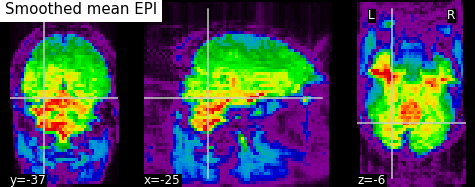
\includegraphics[width=.50\linewidth, height=3cm,  valign=c]{images/epi.png}
    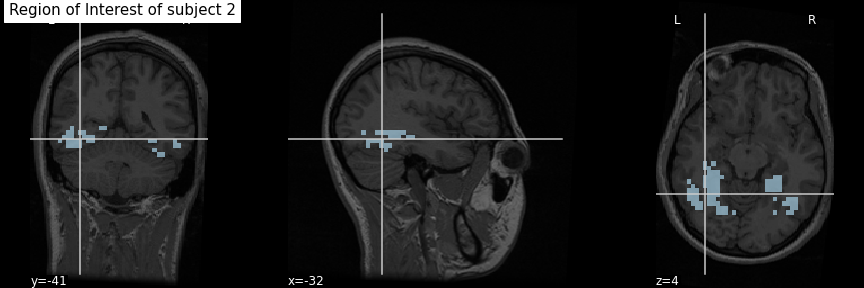
\includegraphics[width=.50\linewidth, height=3cm,  valign=c]{images/roi.png}
    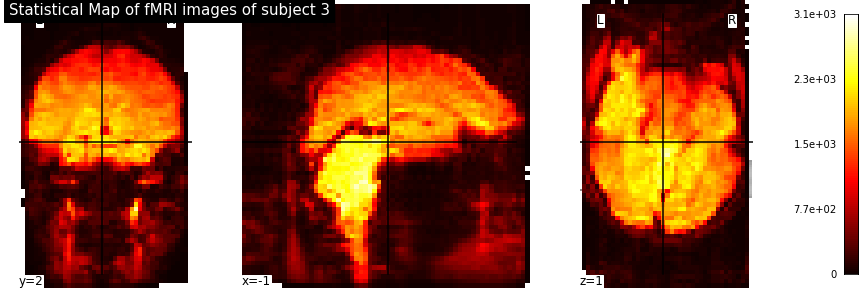
\includegraphics[width=.50\linewidth, height=3cm,  valign=c, valign=c]{images/stats_map.png}
    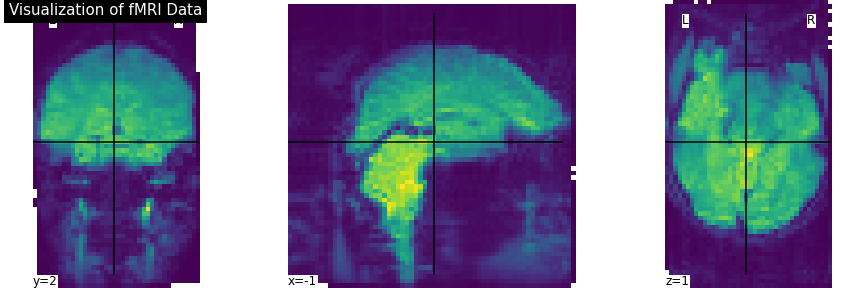
\includegraphics[width=.50\linewidth, height=3cm,  valign=c, valign=c, valign=c]{images/fMRI.png}
    \\[\smallskipamount]
    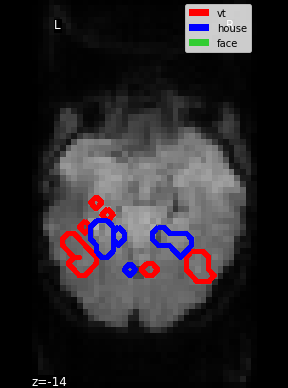
\includegraphics[width=.50\linewidth, height=3cm,  valign=c]{images/pretty_brain_response.png}
    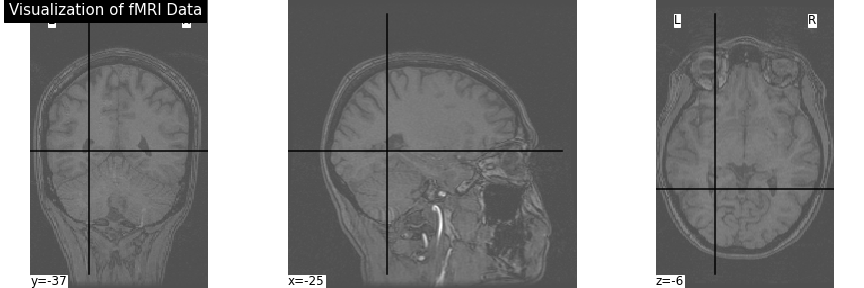
\includegraphics[width=.50\linewidth, height=3cm,  valign=c]{images/anat.png}
    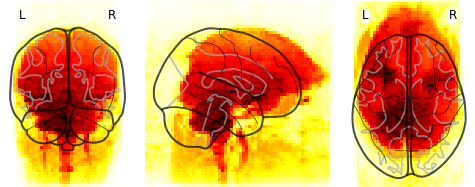
\includegraphics[width=.50\linewidth, height=3cm,  valign=c]{images/glass_brain_white.png}
    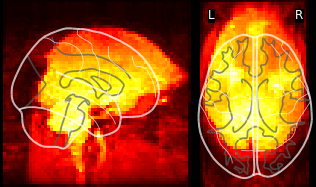
\includegraphics[width=.50\linewidth, height=3cm,  valign=c]{images/glass_brain_black.png}
    \\[\smallskipamount]
    \caption{Visualizations of ventral temporal cortex of subjects with different kinds of neuroimaging technique. From top left to bottom right in sequential way, the visuals corresponds the smoothed temporally average EPI, RoI's, statistical map, direct fMRI, activated regions of brain by some stimulus, anatomical, white and black glass brain visuals of the subjects in the Haxby experiment.}\label{fig:neuroimag}
\end{figure*}



%%%%%%%%% BODY TEXT
\section{Introduction}
The ventral temporal cortex in the human brain is selective to the different representations of the visual stimuli from nature and ventral object vision pathway generates distributed and overlapping neural responses \cite{tanaka1996inferotemporal}. Single cell studies are conducted to demonstrate that the differential tuning of individual neurons in the ventral temporal cortex in nonhuman primates are selective the objects from different kinds and form representative features \cite{gross1972visual, tanaka1996inferotemporal}. However, their order of selectivity is not generalizable and scalable to higher degree of object representations \cite{ds000105:00001}. To model neuro architecture of the ventral cortex, statistical algorithms are developed but the uncertainty in pathway remains. Recent developments regarding neuroimaging have demonstrated that spatio-temporal decoding of human's perception, memories and thoughts are decodable via functional magnetic resonance imaging (fMRI) methods \cite{huang2021fmri}. However, the complexity and the distribution of fMRI data require sophisticated scientific tools because of its neural capacity of the spatio-temporal resolution. With the advancements of machine learning, neuroscientists discover statistical and structural patterns in large scale fMRI datasets to solve various tasks in the context of neuroscience. Further, recent advances in deep learning enable researchers to solve unsolved neuroscientific tasks \cite{koster2018big} and concretely show the importance of deep learning.
In this study, we build an end-to-end discovery machine learning pipelines to decode the category of visual stimuli viewed by a human subject based on fMRI data. Further, we construct vision transformers with spatially oriented attention mechanisms for understanding attention in human brains in depth. We utilize the state-of-the-art explanatory neuroimaging technologies such as echo-planar, region-of-interest (RoI), statistical map, anatomical and glass brain methods, to visualize and pre-analyze the visual structure of fMRI samples. Our ablation studies and experiments are based on a block-designed 4-D timeseries fMRI dataset, namely Haxby dataset \cite{hansoncombinatorial, o2005partially, ds000105:00001}, from the study on face and object representation.


Further, we performed functional connectivity analysis based on the correlation, precision and partial correlation, and similarity analysis based on the cosine, minkowski and euclidean distance to discover overlapping representation in ventral temporal cortex. Then, manifold learning and dimensionality reduction methods are performed on the per-subject ventral temporal masks to extract latent variables of spatio-temporal masks that will help further decoding of human brain. As dimensionality reduction methods, we applied Principal Component Analysis (PCA), Linear Discriminate Analysis (LDA), Independent Component Analysis (ICA), Non-Negative Matrix Factorization (NNMF) and Multidimensional Scaling (MDS) then compare these obtained subspaces by their 3D visualization. Additionally, we performed manifold learning algorithms to extract underlying manifold distribution in masked ventral temporal regions. We performed t-Stochastic Neighbour Embedding (t-SNE), Uniform Manifold Approximation and Projection (UMAP), ISOMAP, Locally Linear Embedding (LLE) and Spectral Embedding (SE) then compare their lower dimensional manifolds by their 3D visualizations that further help in the decoding process.

\begin{figure*}
    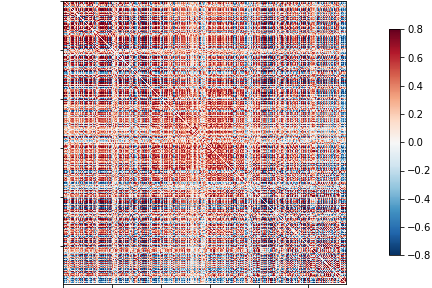
\includegraphics[width=.35\linewidth, height=4cm,  valign=c]{images/correlation.png}
    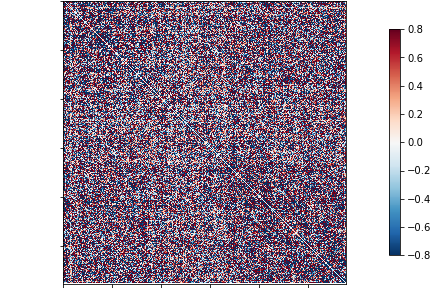
\includegraphics[width=.35\linewidth, height=4cm,  valign=c]{images/precision.png}
    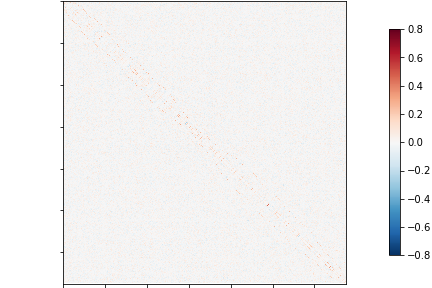
\includegraphics[width=.35\linewidth, height=4cm,  valign=c, valign=c]{images/partial_correlation.png}
    \caption{Functional Connectivity analysis on ventral temporal masks of the subjects are performed with correlation, precision and partial correlation measures in sequential way from left to right.}\label{fig:functional}
\end{figure*}

\begin{figure*}
     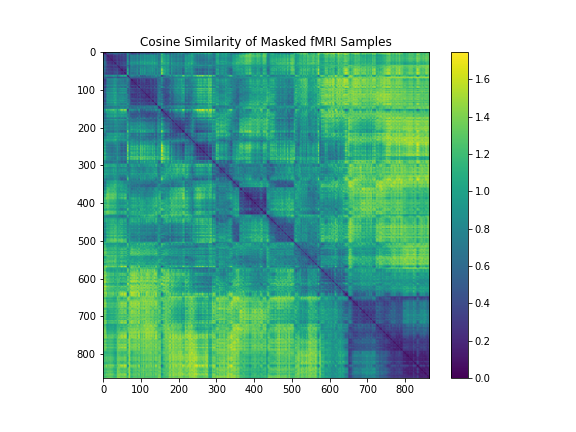
\includegraphics[width=.35\linewidth, height=6cm,  valign=c]{images/cosine.png}
    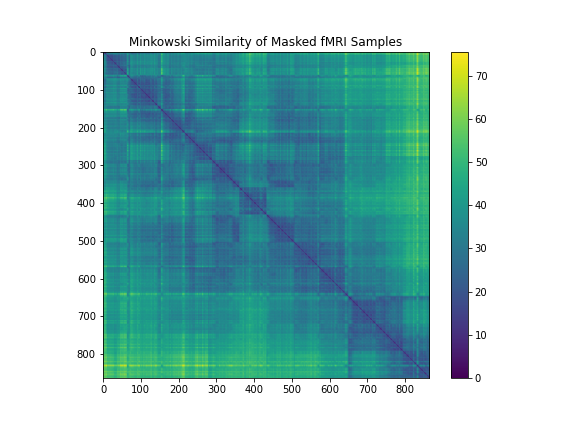
\includegraphics[width=.35\linewidth, height=6cm,  valign=c]{images/minkowski.png}
    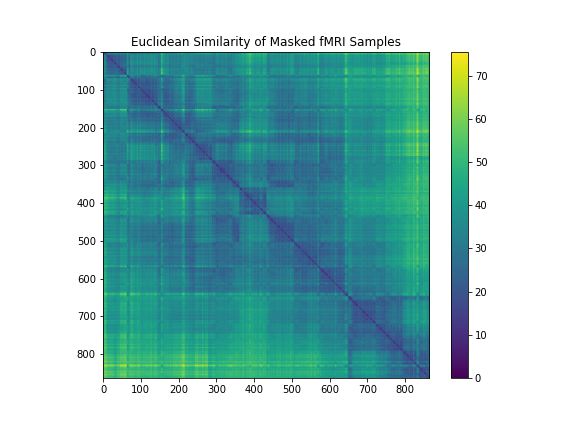
\includegraphics[width=.35\linewidth, height=6cm,  valign=c]{images/euclidean.png}
    \caption{Similarity analysis on ventral temporal masks of the subjects are performed with cosine, minkowski and euclidean distance in sequential way from left to right.}\label{fig:sim}
\end{figure*}

\begin{figure*}
     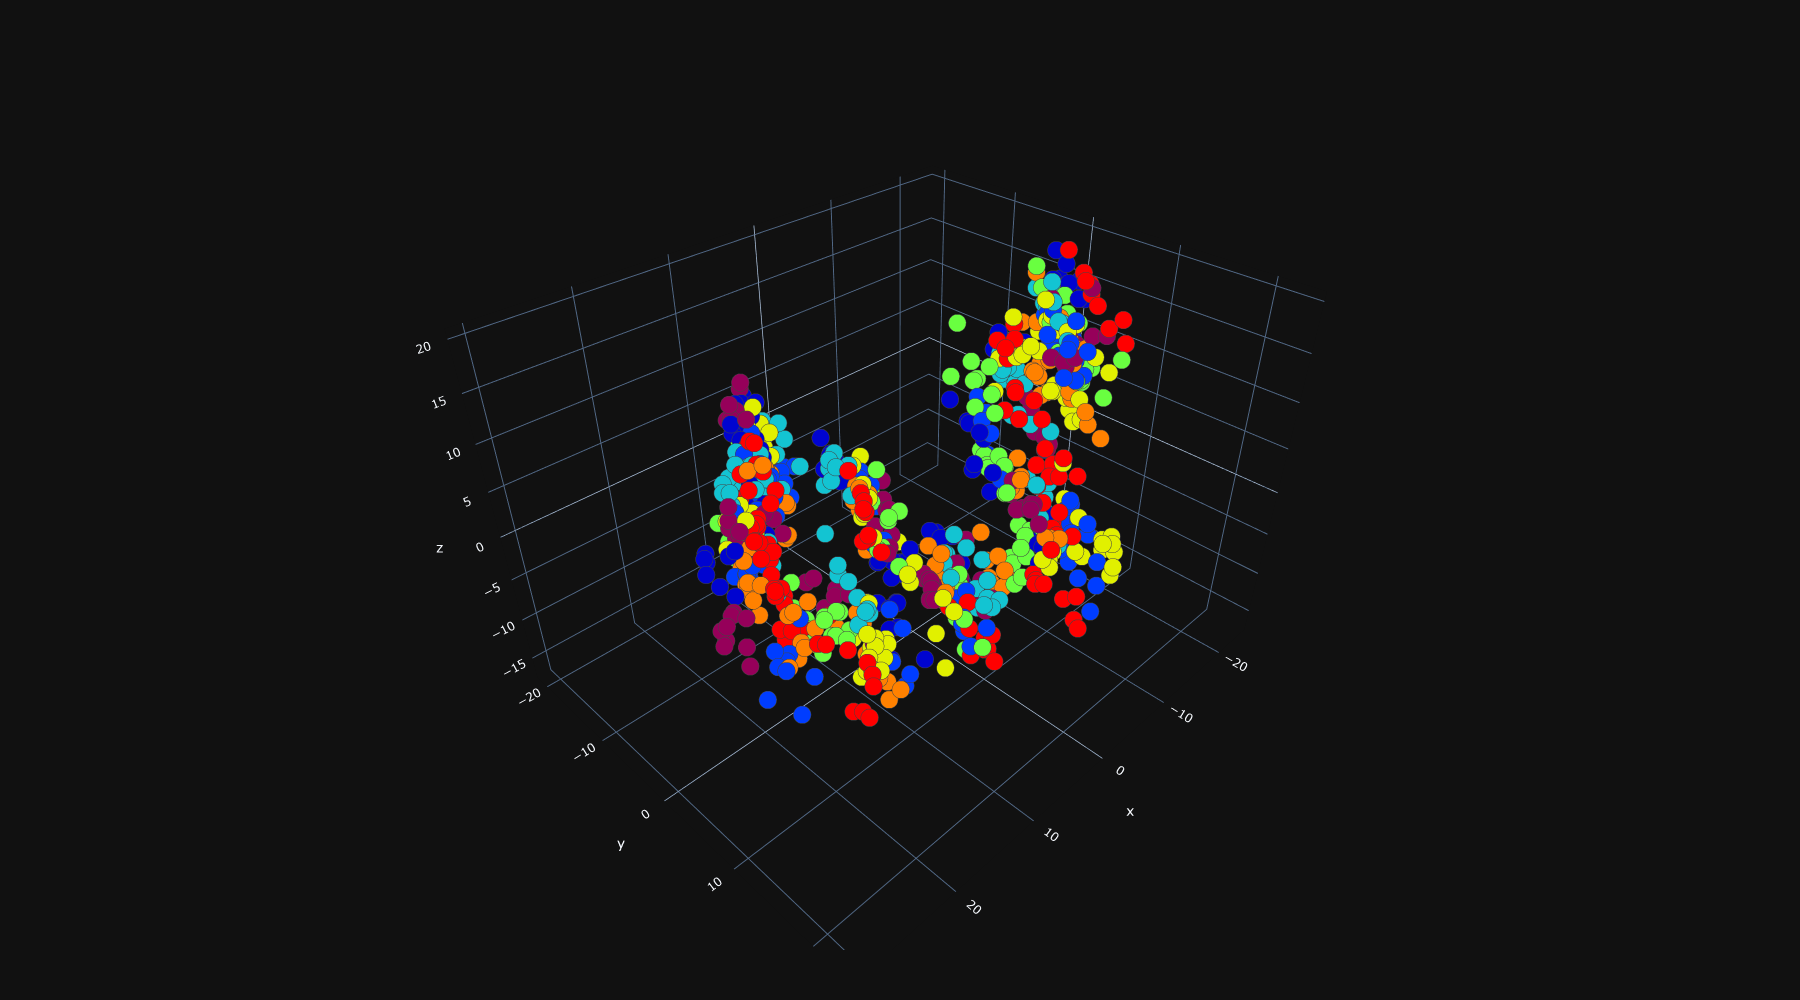
\includegraphics[width=.33\linewidth, height=6cm,  valign=c]{images/pca_3d.png}
    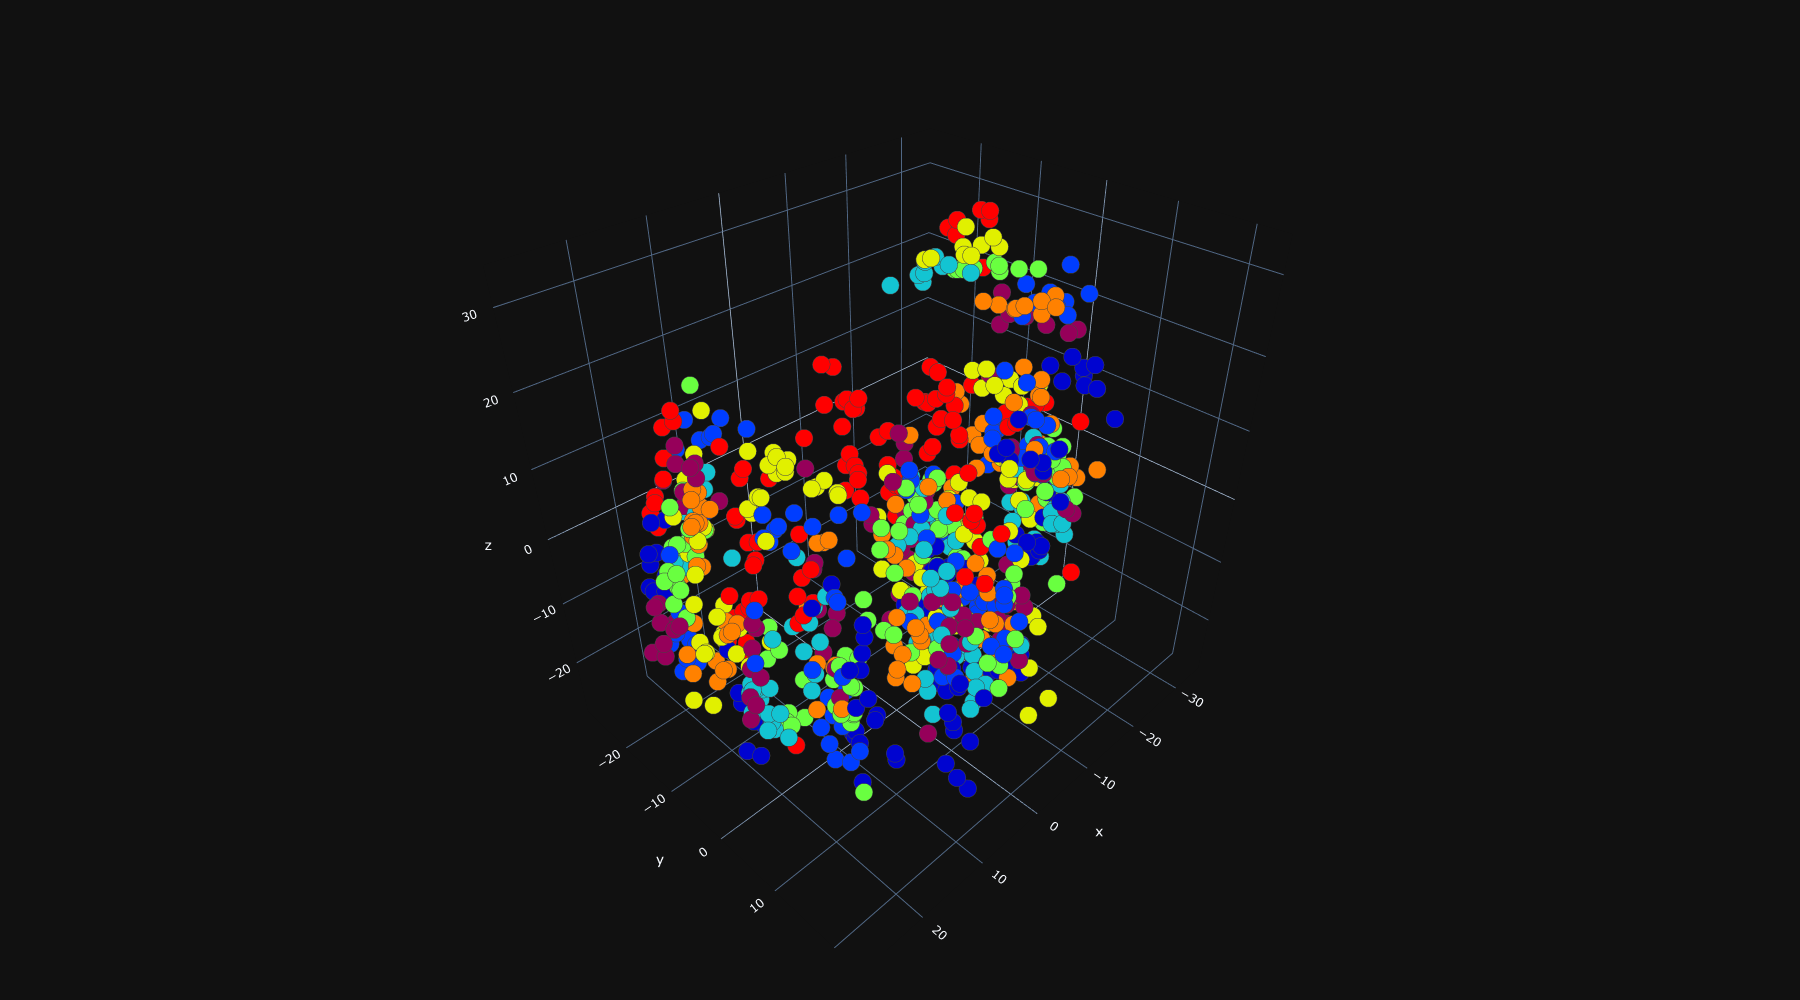
\includegraphics[width=.33\linewidth, height=6cm,  valign=c]{images/mds_3d.png}
    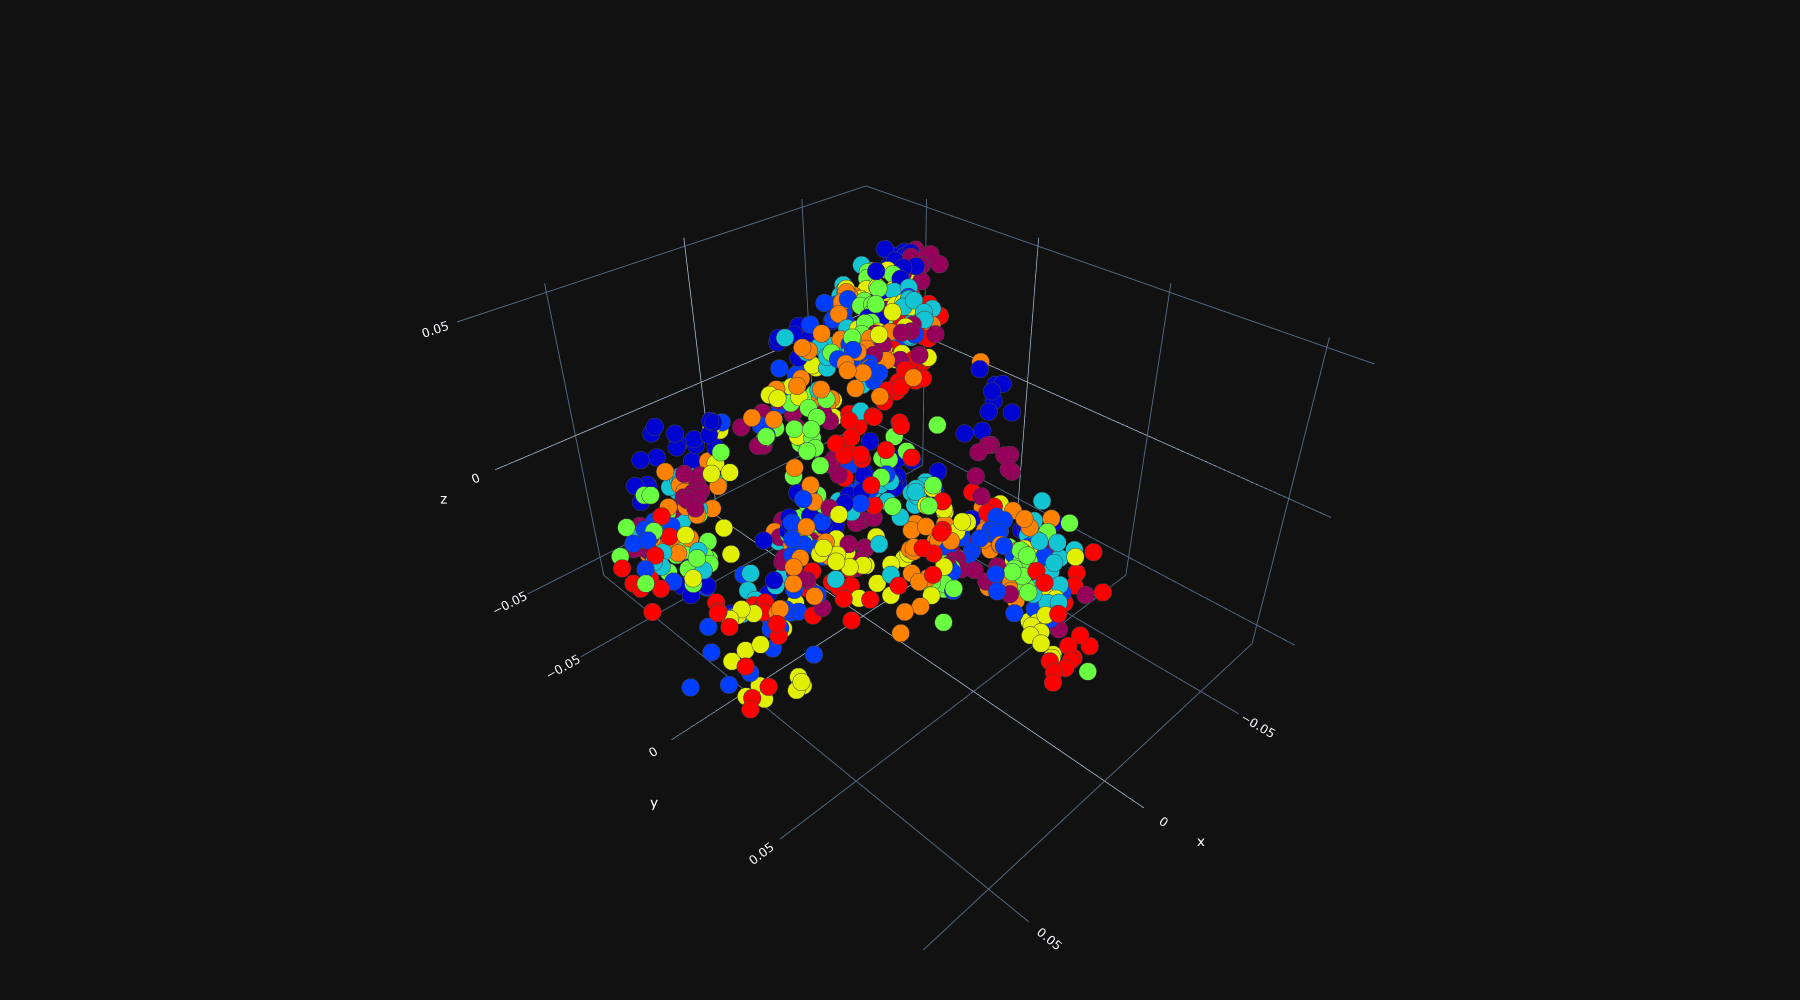
\includegraphics[width=.33\linewidth, height=6cm,  valign=c]{images/ica_3d.png}
    \\[\smallskipamount]
    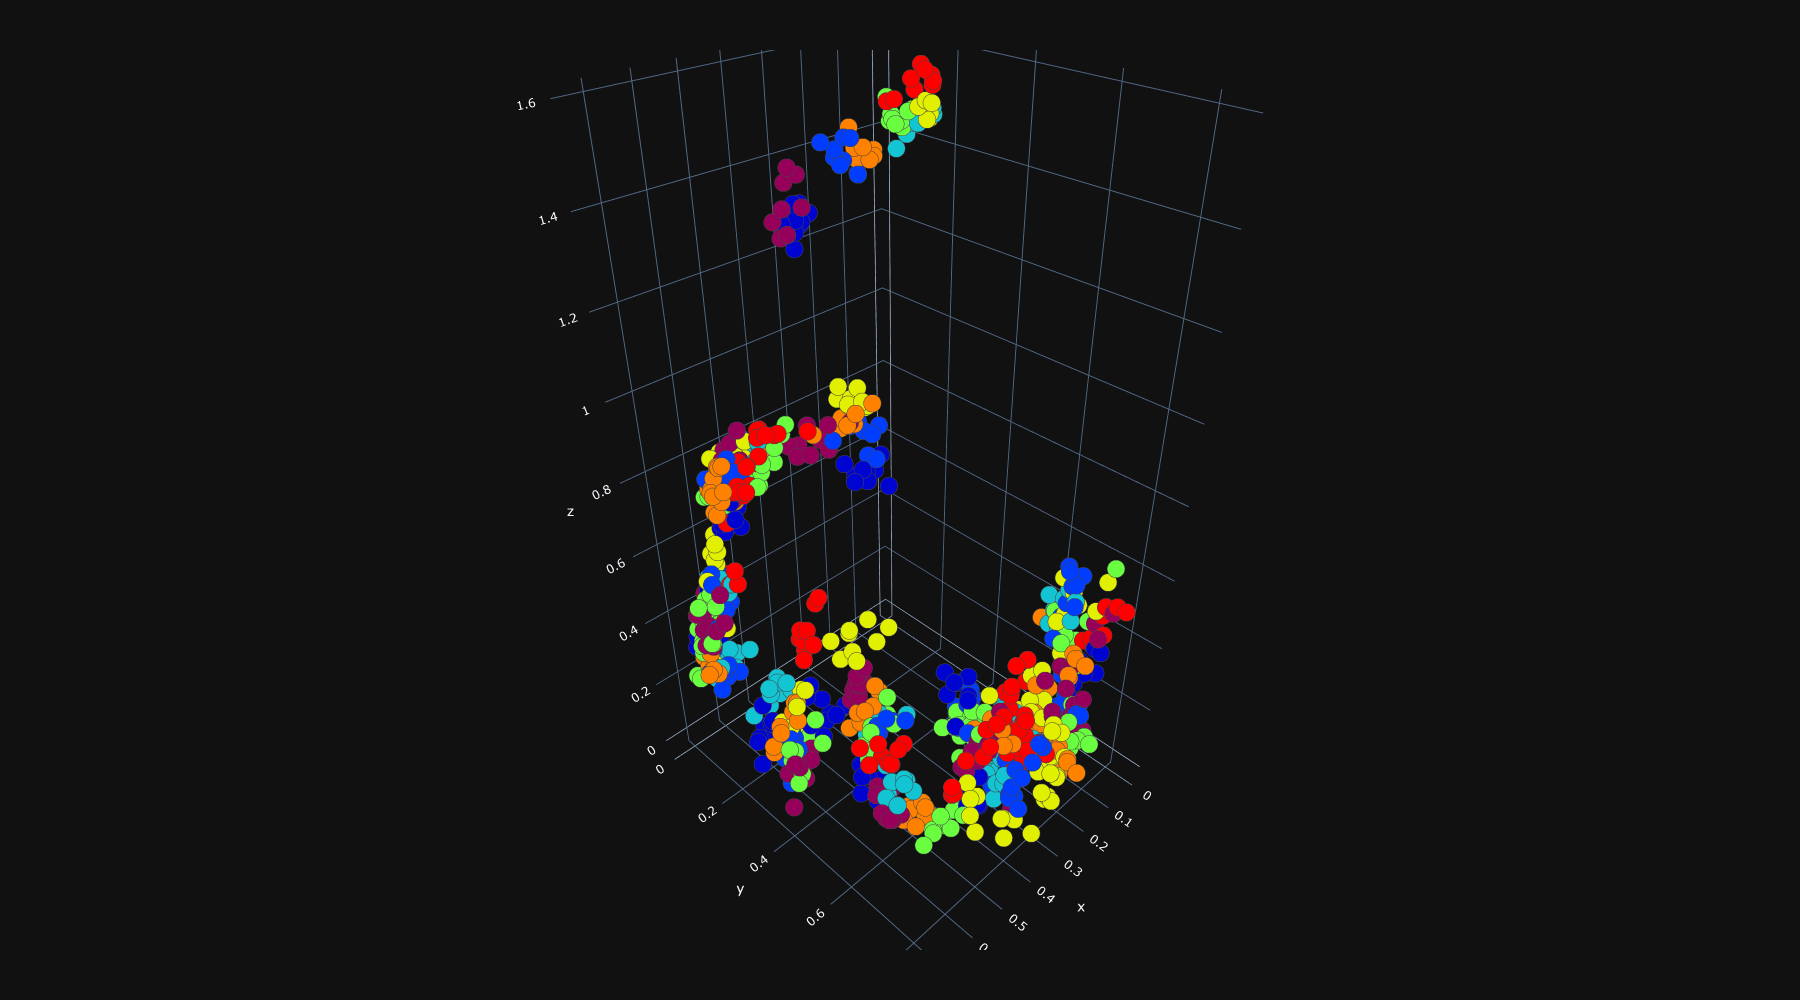
\includegraphics[width=.5\linewidth, height=4cm,  valign=c]{images/nnmf_3d.png}
    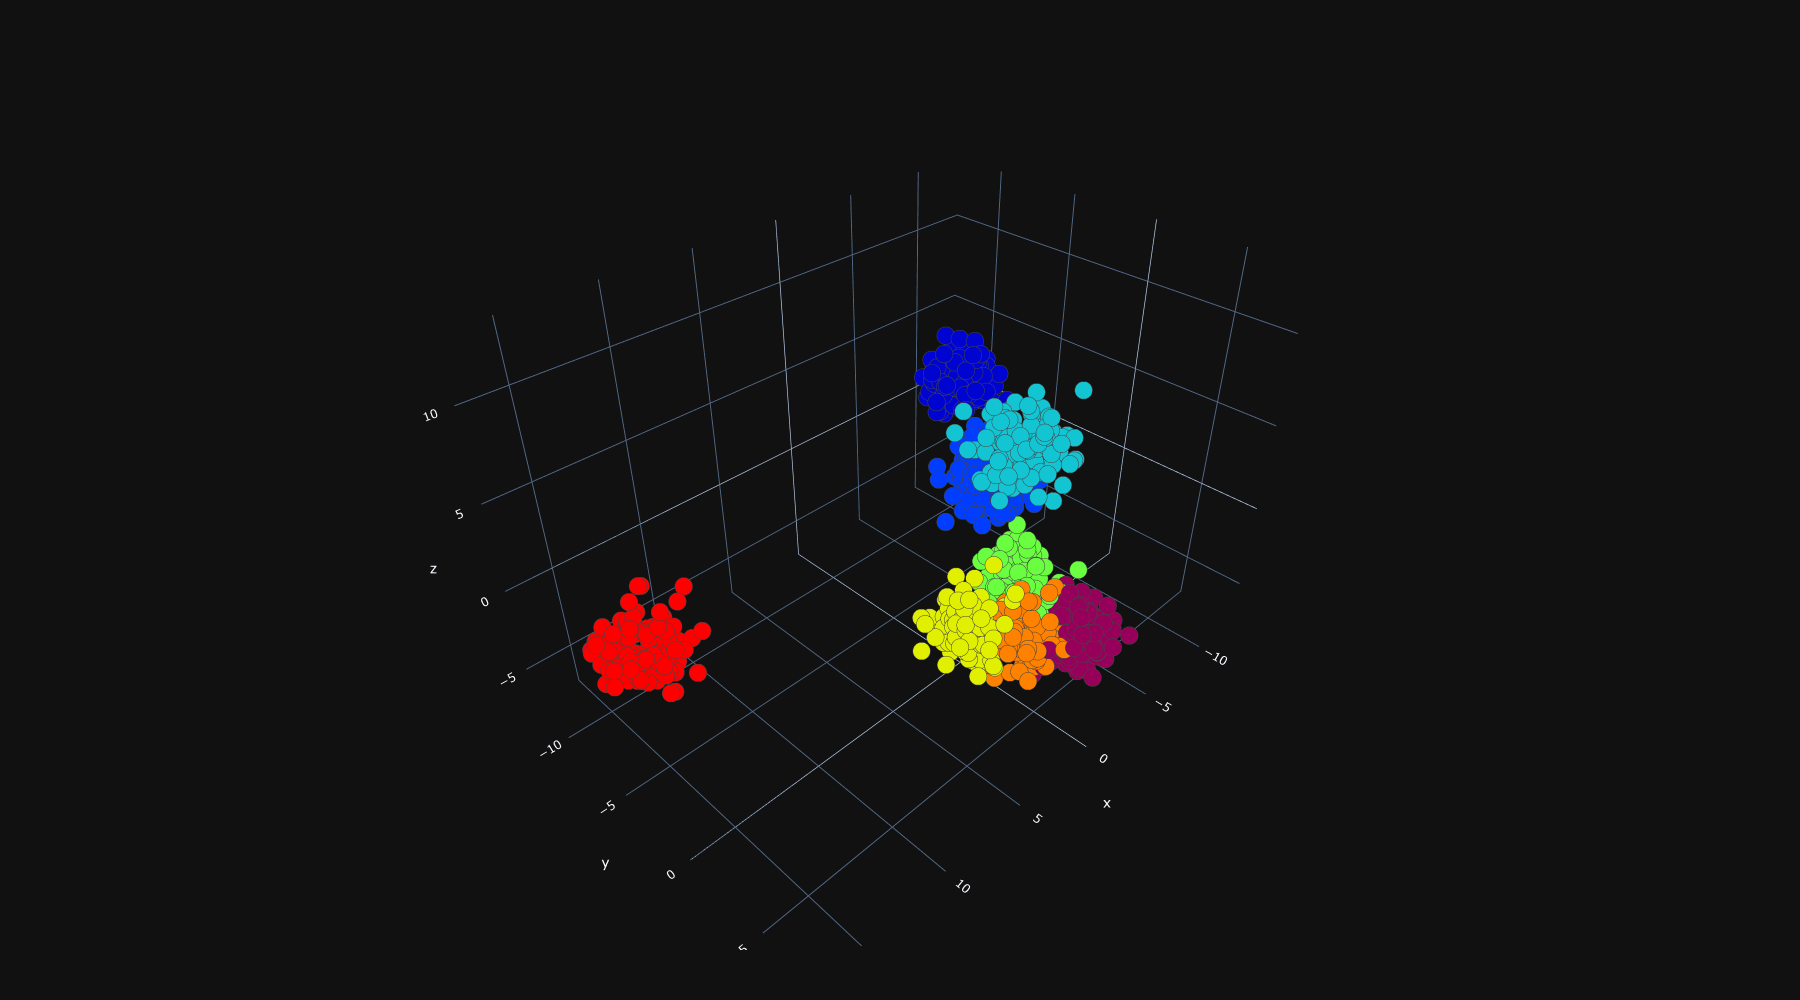
\includegraphics[width=.5\linewidth, height=4cm,  valign=c]{images/lda_3d.png}
    \caption{Dimension reduction algorithms: PCA, MDS, ICA, NNMF and LDA are performed with 3 component for visualization purposes that are presented in sequential way from top left to bottom right. Unique colors represent unique classes.}\label{fig:dim}
\end{figure*}


\begin{figure*}
     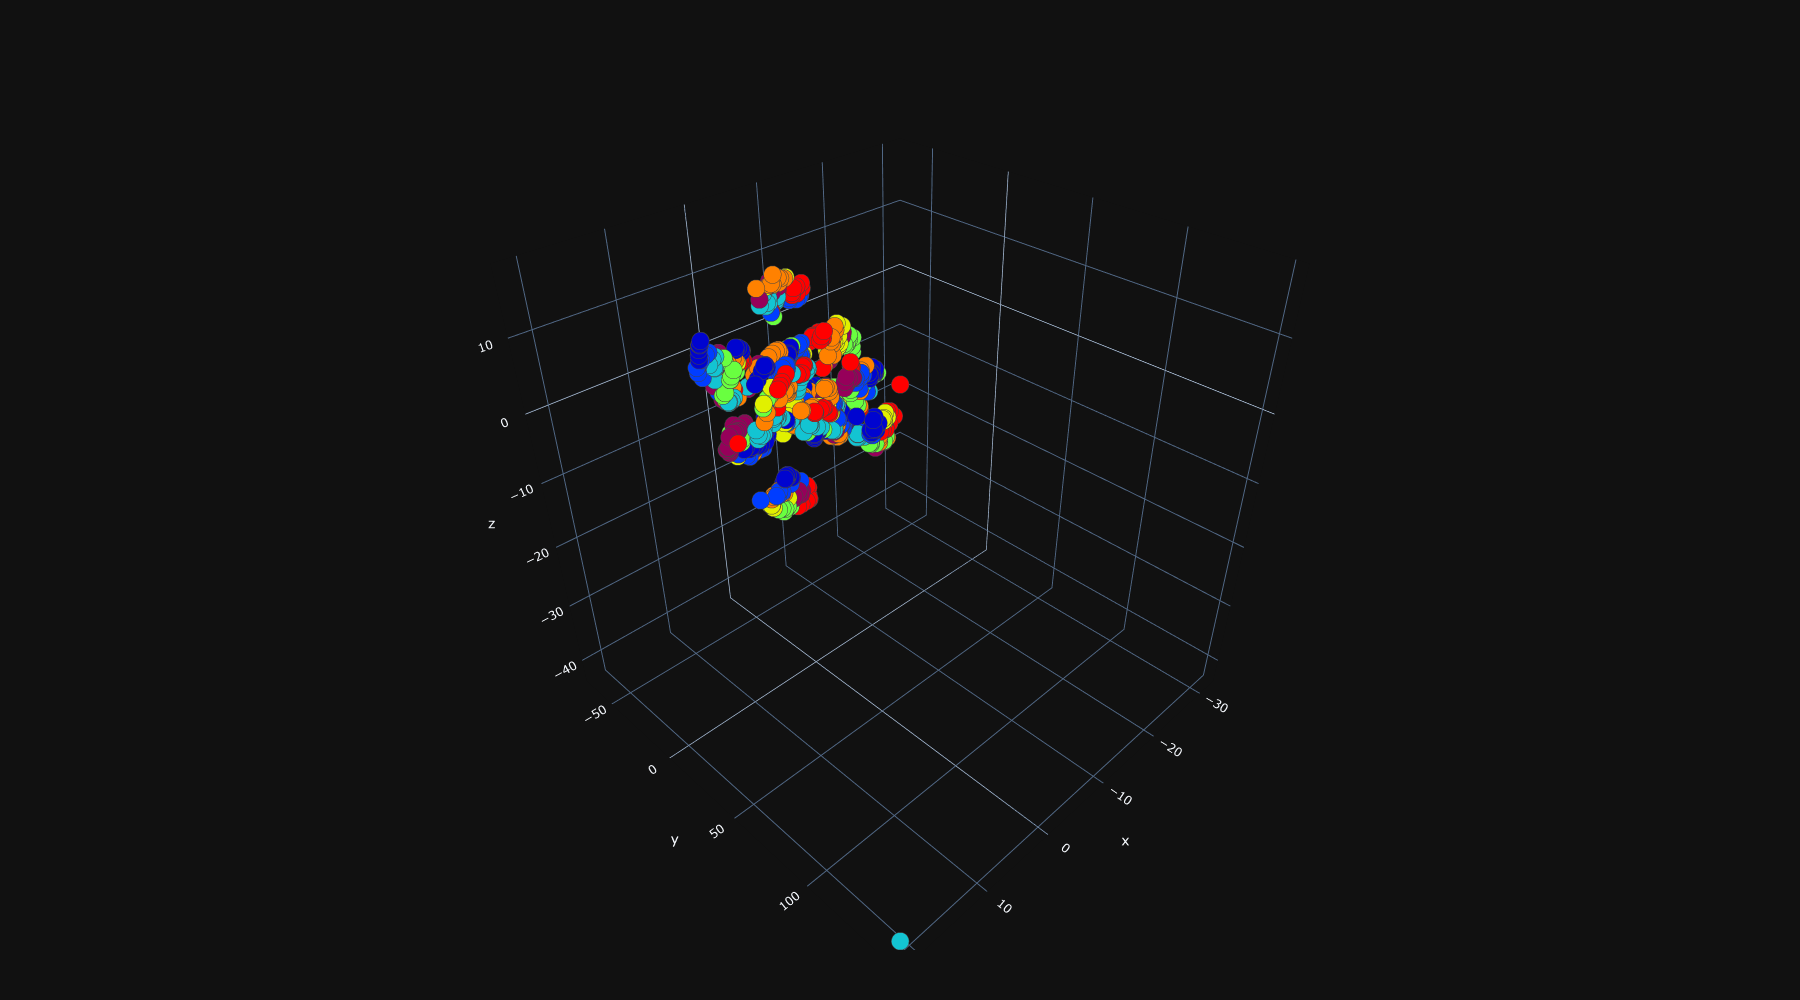
\includegraphics[width=.33\linewidth, height=6cm,  valign=c]{images/tsene_3d.png}
    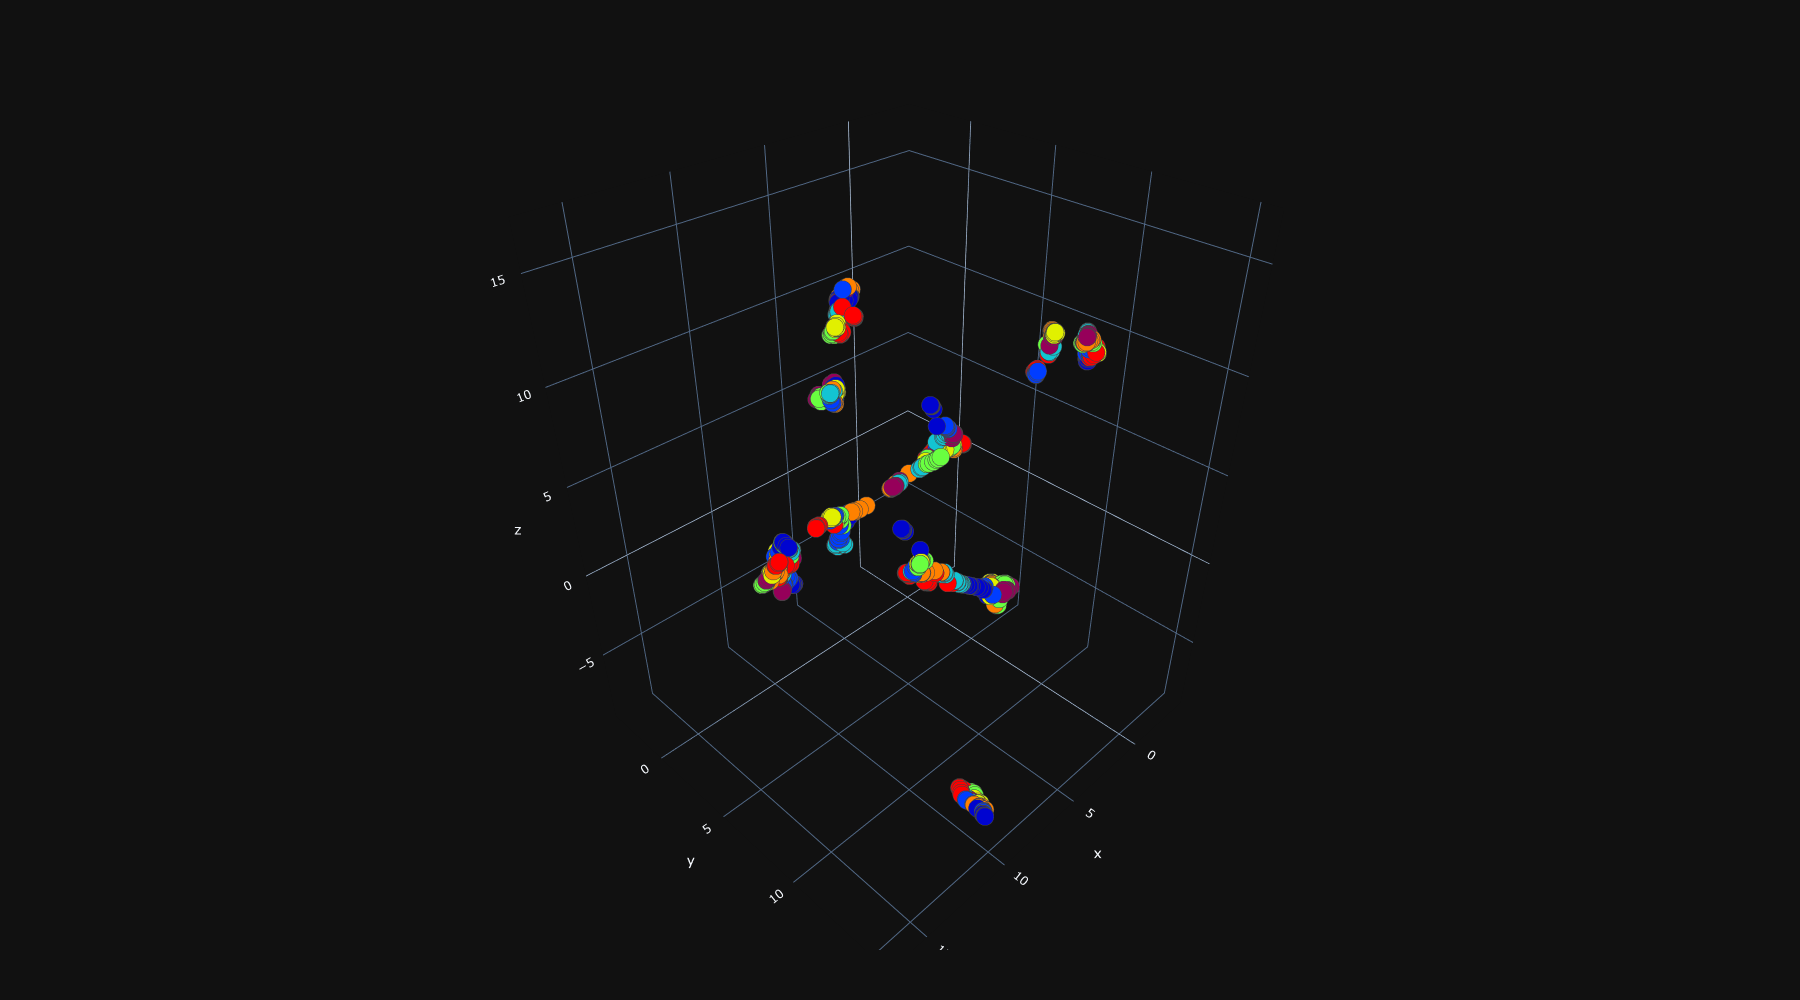
\includegraphics[width=.33\linewidth, height=6cm,  valign=c]{images/umap_3d.png}
    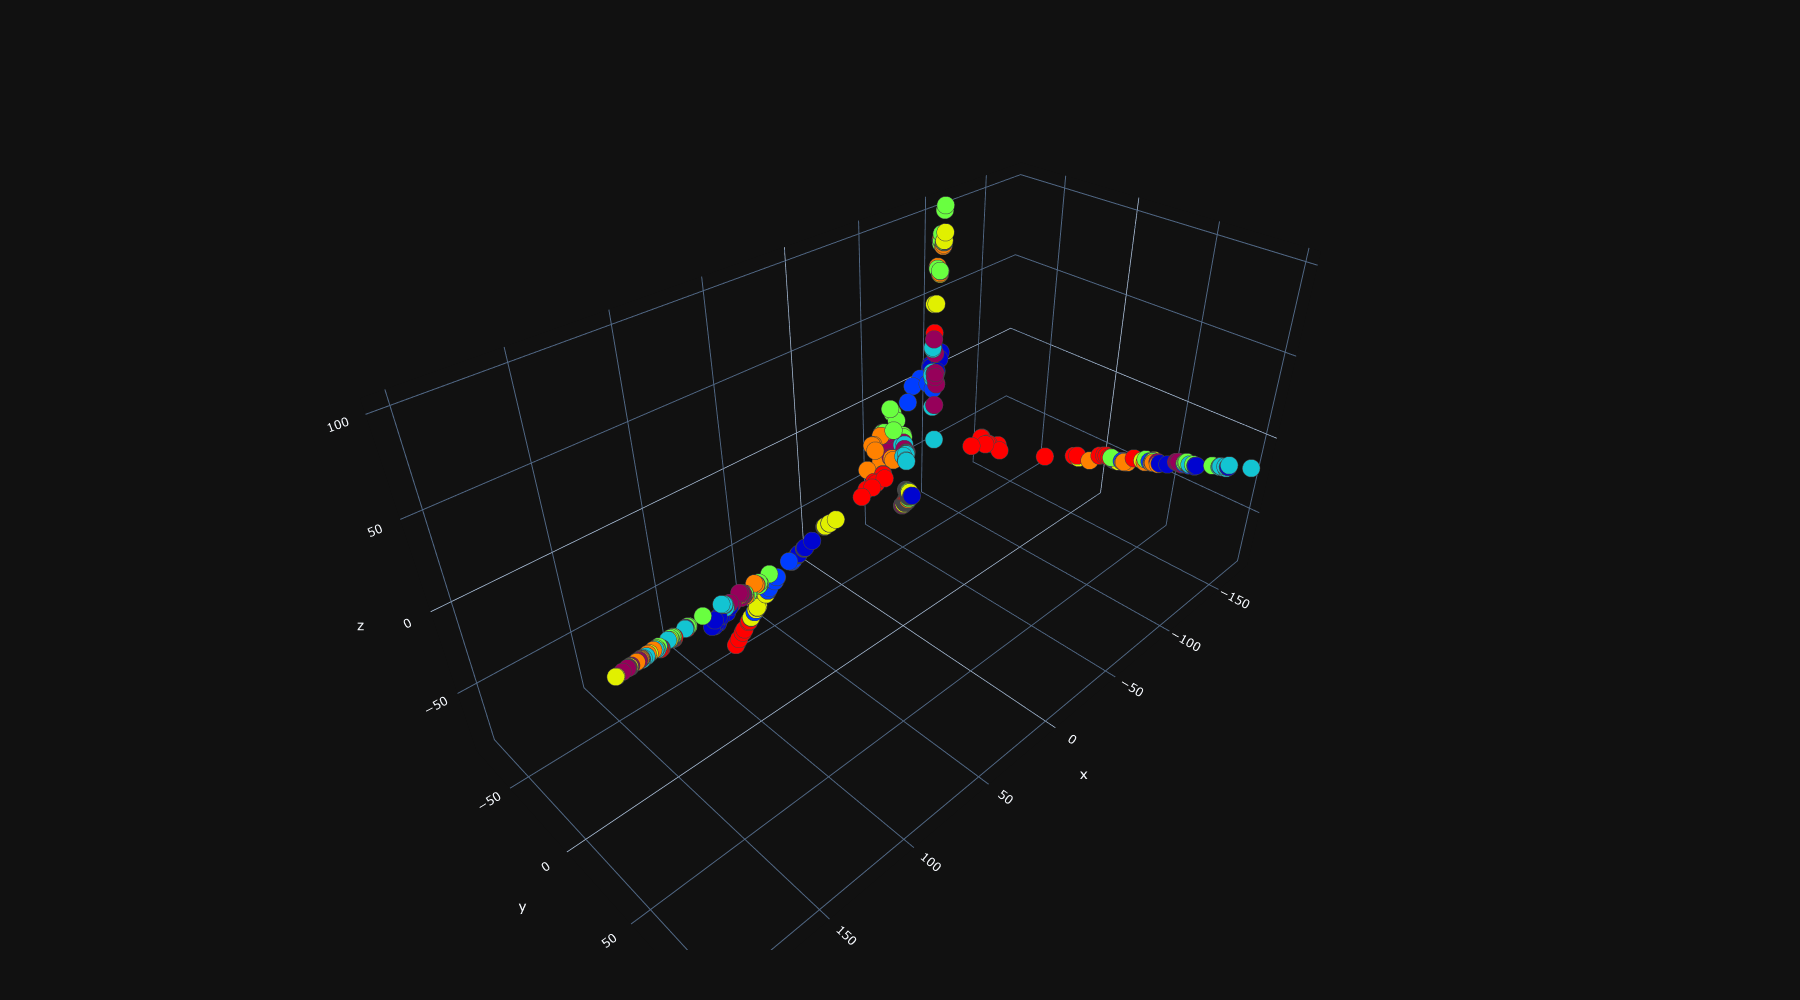
\includegraphics[width=.33\linewidth, height=6cm,  valign=c]{images/isomap_3d.png}
    \\[\smallskipamount]
    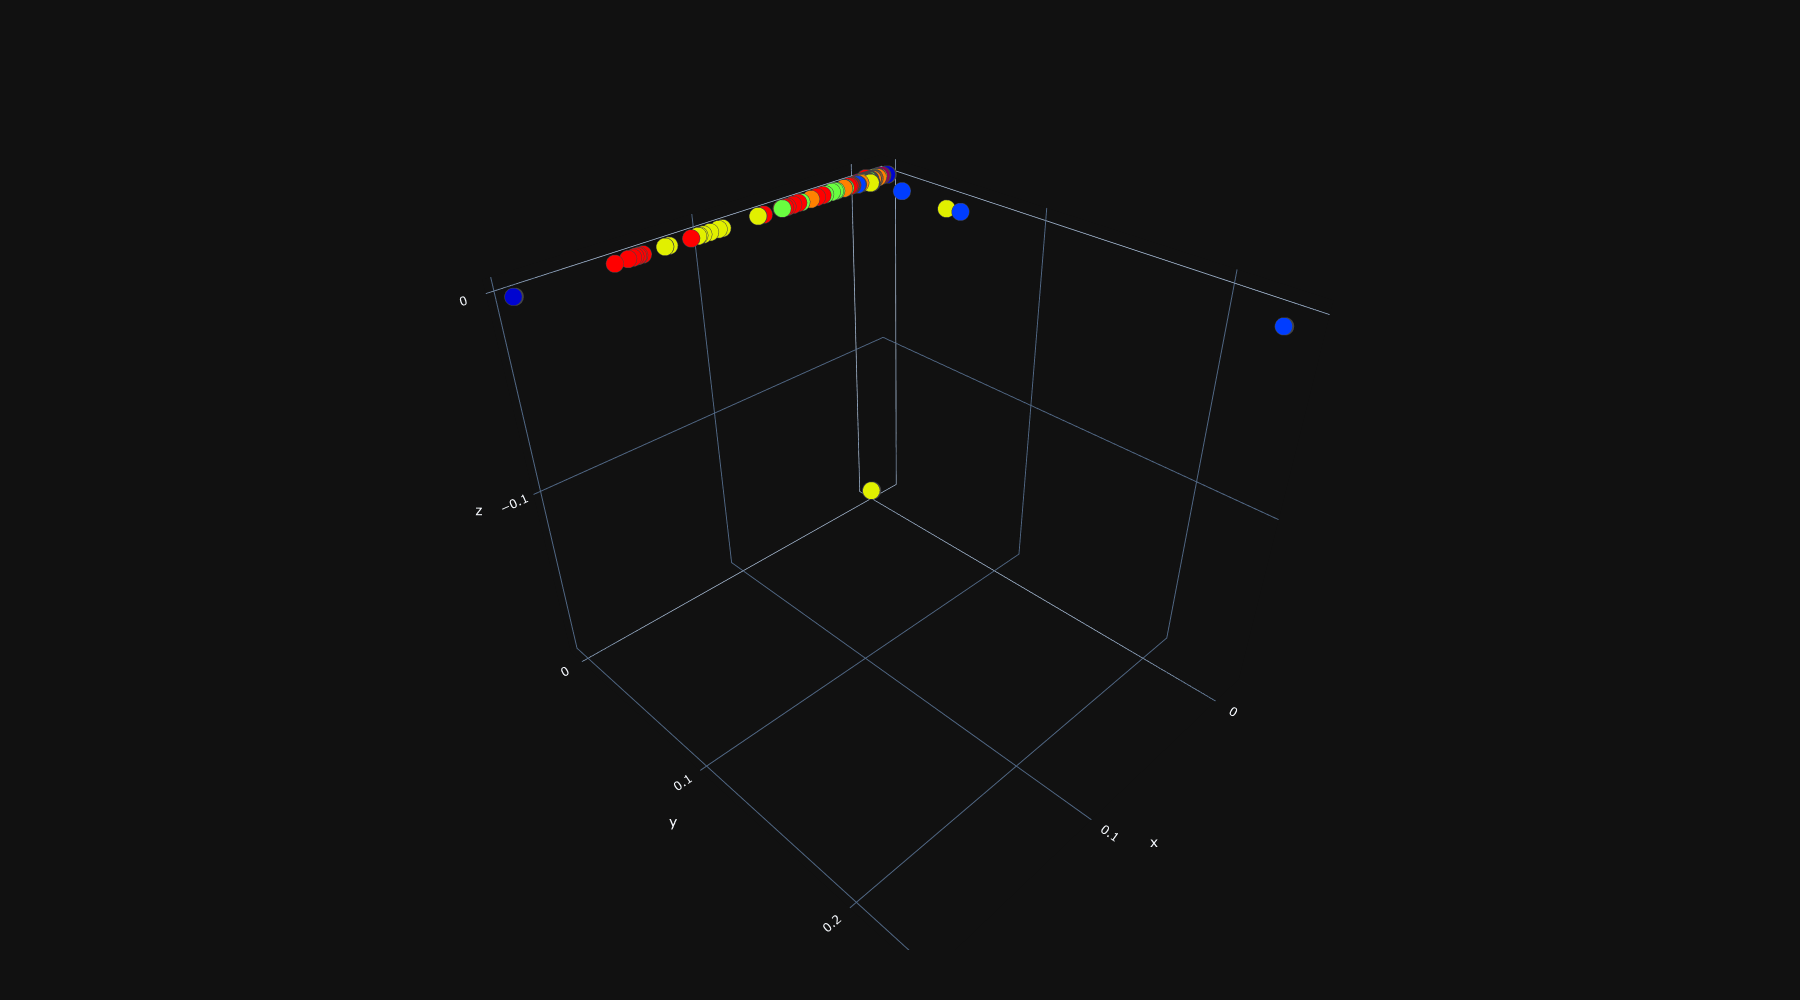
\includegraphics[width=.5\linewidth, height=4cm,  valign=c]{images/lle_3d.png}
    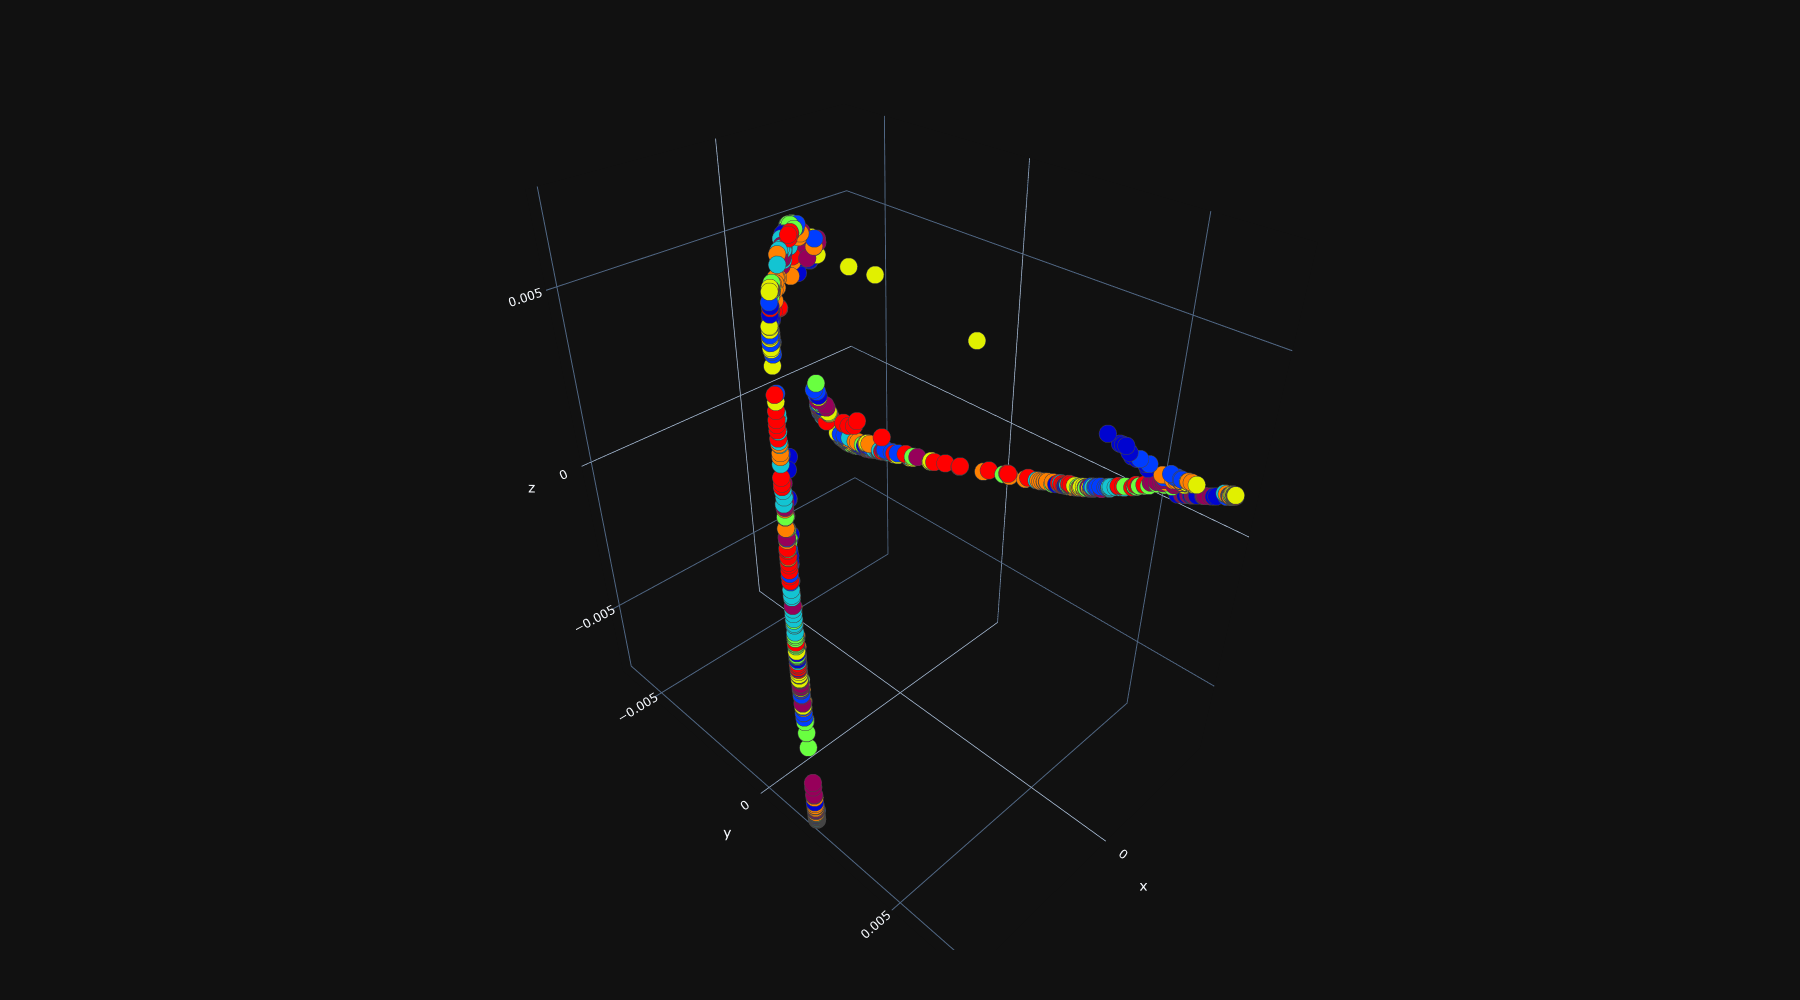
\includegraphics[width=.5\linewidth, height=4cm,  valign=c]{images/SpectralEmbedding_3d.png}
    \caption{Manifold learning: t-SNE, UMAP, ISOMAP, LLE and Spectral Embedding are performed with 3 component for visualization purposes that are presented in sequential way from top left to bottom right. Unique colors represent unique classes.}\label{fig:man}
\end{figure*}


End-to-end machine learning algorithms are developed to categorize the stimuli based on distributed and overlapping regions in the ventral temporal cortex. Precisely, we performed the following machine learning algorithms; Linear support vector classifier (LinearSVC), Stochastic Gradient Descent Classifier (SGDClassifier), Multi-Layer-Perceptron (MLP), Perceptron, Logistic Regression, Logistic Regression Cross-Validation, Support Vector Classifier (SVC), Calibrated Classifier (Probability calibration with isotonic regression), Passive Aggressive Classifier, Label Propagation Classifier, Random Forest Classifier, Gradient Boosting Classifier, Quadratic Discriminant Classifier, Ridge Classifier Cross-Validation, Ridge Classifier, AdaBoost Classifier, Extra Trees Classifier, K-Neighbors Classifier, Bernoulli Naive Bayes Classifier, Gaussian Naive Bayes Classifier, Nu-Support Vector Classifier, Nearest Centroid Classifier and Bagging Classifier. As a robust ensemble decoding, we applied novel ensemble of regularized models; FREM: Cross-Validated Ensemble of L2 regularized SVCs, FREM: Cross-Validated Ensemble of L2 regularized Logistic Regressions. We further constructed cognitive neural networks, precisely MLPs with GELU non-linearity \cite{hendrycks2020gaussian}, 2D and 3D  Convolutional Neural Network and spatially oriented vision transformers by taking the advantage of interactions between different streams of visual representations.

Our main study decomposed as follows.
\begin{itemize}[noitemsep]
    \item We build an end-to-end discovery machine learning and deep learning pipelines to decode the category of visual stimuli viewed by a human subject based on fMRI data. 
    
    \item We utilize state-of-the-art explanatory neuroimaging technologies such as echo-planar, region-of-interest (RoI), statistical map, anatomical and glass brain methods, to visualize and pre-analyze the visual structure of fMRI samples.
    
    \item Further, we performed functional connectivity analysis based on the correlation, precision and partial correlation, and similarity analysis based on the cosine, minkowski and euclidean distances to discover overlapping representation in the ventral temporal cortex.
    
    \item Then, manifold learning and dimensionality reduction methods are performed on the per-subject ventral temporal masks to extract latent variables of spatio-temporal masks.
\end{itemize}


The rest of the paper is organized as follows. We begin with the methods section that we explained methodology from unsupervised representation learning, functional connectivity analysis to machine \& deep learning pipelines. Then, we present our findings, mainly results of the decoding process in terms of widely used evaluation metrics in the results section. Then, we interpret our results in light of previous studies in the discussion section. 

%-------------------------------------------------------------------------
\section{Methods}

Our experiments are based on a block-designed 4-D timeseries fMRI dataset, namely Haxby dataset \cite{hansoncombinatorial, o2005partially, ds000105:00001}, from the study of face and object representation. It consists of 6 subjects with 12 runs per subject \cite{ds000105:00001}. In each run, the subjects passively viewed grey-scale images of eight object categories, grouped in 24s blocks separated by rest periods \cite{ds000105:00001,hansoncombinatorial}. Each image was shown for 500ms and was followed by a 1500ms inter-stimulus interval \cite{hansoncombinatorial}. Full-brain fMRI data were recorded with a volume repetition time of 2.5s, thus, a stimulus block was covered by roughly 9 volumes \cite{ds000105:00001}. It consist of per-subject high resolution anatomical images except for the sixth, 4D fMRI timeseries image data in the shape of $1452$ volumes with $40$x$64$x$64$ voxels (corresponding to a voxel size of 3.5 x 3.75 x 3.75 mm and a volume repetition time of 2.5 seconds) \cite{ds000105:00001}. We have 8 different stimuli categories that are scissors, face, cat, scrambledpix, bottle, chair, shoe and house. The visuals of stimuli is presented in appendix \ref{appendix:A}. The chunks of resting-state is eliminated as it provides no additional information on decoding visual stimuli \cite{ds000105:00001}.  We performed multiple explanatory and decoding experiments. In the following sections, we described our methodology in detail. We started with discovery and advanced visualizations of ventral temporal cortex by different neuroimaging techniques, their underlying manifolds, functional connectome analysis of overlapping regions, and we provide descriptions of more than 30 ML \& DL brain decoders.

\subsection{Discovery fMRI Analysis by Neuroimaging}
We performed pre-analysis based on the neuroimaging technologies to visualize the dataset. To accomplish that, we utilized the Echo-planar Averaging for 4-D visualization, region of interest (RoI), statistical map, anatomic, glass brain visualization tools embedded in statistical learning and neuroimaging framework, namely Nilearn \footnote{\url{https://nilearn.github.io/}}. 

\subsubsection{Echo-Planar Imaging for 4-D Visualization of the fMRI}
Echo-planar imaging is a very fast magnetic resonance (MR) imaging technique capable of acquiring an entire MR image in only a fraction of a second \cite{poustchi2001principles}. In single-shot echo-planar imaging, all the spatial-encoding data of an image can be obtained after a single radio-frequency excitation \cite{poustchi2001principles}. Here, we visualize the EPI for subjects of the Haxby experiment from cuts of frontal, axial and lateral regions in figure \ref{fig:epi} in appendix \ref{appendix:B}. EPI visualization provides realistic insights from the activated regions in the brain that plays a crucial role in spatio-temporal brain decoding.


\subsubsection{Region of Interest Analysis}
A common way to analyze fMRI data is performing the region of interest (RoI) analysis that involves the extraction of signals from specified areas. The most theoretically agnostic use of ROI analysis is to simply explore the underlying signal behind a whole-brain voxel-wise analysis \cite{poldrack2007region}. After extracting statistically meaningful areas, we can perform severity of correction for multiple statistical tests instead of large number of voxels in brain. Sample RoI visualization is performed, can be found at figure \ref{fig:neuroimag}. In the top right corner, we visualized the RoI for subject 2 in Haxby dataset. Further, most ML decoders are performed on the RoI's of subjects instead of whole brain medium.

\subsubsection{Statistical Maps}
Statistical Parametric Mapping refers to the construction and assessment of spatially extended statistical processes used to test hypotheses about functional imaging data \cite{friston1994statistical}. Generally, the prior step in statistical fMRI is to create a thresholded statistical map, representing the regions that are active (above a threshold) \cite{poldrack2007region}. Hence, it is useful in examining differences in brain activity recorded during neuroscientific experiments. Here, we performed statistical mapping and visualized it in the figure \ref{fig:neuroimag}. In the second above left figure, we visualized the statistical map of subject 3 with threshold value 3.


\subsubsection{Direct fMRI Visualizations}
Simple and compact visualization of fMRI data is quite important topic in the context of neuroimaging since it enables researchers to view cortical brain activity. So, we directly plot the temporally averaged fMRI data of subject 2 to further visualization. It can be found at figure \ref{fig:neuroimag} in the second above right part of the figure.


\subsubsection{Anatomic Visualizations}
We visualized the anatomical structure of the fMRI (by default 3 cuts: Frontal, Axial, and Lateral) obtained by the temporally averaged fMRI data of the subject 2 to generate insights before decoding in figure \ref{fig:neuroimag} at the second above left part of the figure. % add something here 


\subsubsection{Glass Brain}
The Glass Brain is a state-of-the-art real-time brain visualization technology that is created on the Unity 3D game-engine and powered by NVIDIA’s GPU computing \cite{reddy2021pilot}. Its inputs include an individual’s brain structure, both tissue and fiber tract architecture, obtained from high-resolution MRI-DTI brain scans. Real-time brain activity and functional interactions among networks are superimposed on the brain structure using high-density EEG (electroencephalography) \cite{reddy2021pilot}. Here, we project frontal, axial, and lateral sides of temporally averaged fMRI data of subject 5 and visualized it in figure \ref{fig:neuroimag}. The last row of the figure \ref{fig:neuroimag} represents the glass brain visualizations. 

\subsection{Functional Connectivity and Similarity Analysis}
Functional connectivity is defined as the temporal dependency of neuronal activation patterns of anatomically separated brain regions and in the past years an increasing body of neuroimaging studies has started to explore functional connectivity by measuring the level of co-activation of resting-state fMRI time-series between brain regions \cite{van2010exploring}. These functional connections are important in establishing statistical connections in brain regions. Functional connectivity can be obtained by estimating a covariance (or correlation) matrix for signals from different brain regions decomposed, for example on resting-state or naturalistic-stimuli datasets. Here, we performed functional connectivity analysis based on the correlation, precision and partial correlation. Then, similarity analysis based on the cosine, minkowski and euclidean distance is performed to further extend statistical findings in masked fMRI data. Please refer to self-explained figures \ref{fig:functional} and \ref{fig:sim} for depth understanding.    


\subsubsection{Functional Connectivity: Correlation}
Functional connectivity based on Pearson correlation is performed on subject 1 and visualized in figure \ref{fig:functional} at top left corner. We can see that in the ventral temporal cortex of subject 1, there are correlations when the stimuli of faces are presented. 

\subsubsection{Functional Connectivity: Precision}
As shown in the papers \cite{smith2011network, varoquaux2010brain}, it is more interesting to use the inverse covariance matrix, i.e. the precision matrix. It gives only direct connections between regions, as it contains partial covariances, which are covariances between two regions conditioned on all the others. Moreover, we performed functional connectome based on precision score, to extract signals on RoI's of subject 1 and visualized in the figure \ref{fig:functional} at top center. Here, with the change in the connectivity measure, we see direct changes in spatial correlations in the ventral cortex of subject 1. With precision measure, we further get understanding in brain organization and brain networks. 

\subsubsection{Functional Connectivity: Partial Correlation}
Among the range of network modeling methods, partial correlation has shown great promises in accurately detecting true brain network connections \cite{wang2016efficient}. So, we performed functional connectivity analysis based on partial correlation and visualized it in figure \ref{fig:functional} at top right corner. Visualization of partial correlation in RoI fMRI data demonstrate that the ventral temporal cortex of the subject 1 is not much correlated.  

\subsubsection{Similarity Analysis: Cosine Similarity}
To facilitate the geodesic understanding in the context of statistical connections in the brain, we performed cosine similarity analysis on subject 1, and the obtained matrix is visualized in figure \ref{fig:sim} at the lower left corner. The results demonstrate that there are highly overlapping regions in terms of neural activity when visual stimuli is presented. 

\subsubsection{Similarity Analysis: Minkowski Similarity}
To experiment with different similarity metrics, we utilized the minkowski distance that is a generalization of both the Euclidean and the Manhattan distance. Hence, it is useful in fMRI temporal similarity analysis.

\subsubsection{Similarity Analysis: Euclidean Similarity}
Lastly, we performed similarity analysis based on classical euclidean distance. It is a very classical measure of the distance in terms of cartesian coordinates of the points using the Pythagorean theorem \cite{maor2019pythagorean}. From the statistical and structural patterns exposed by functional connectivity and similarity analysis, we can conclude that the neural activity evoked in the ventral temporal cortex of the human brain is highly overlapping and distributed.  

\subsection{Dimension Reduction to Manifold Learning}
Functional MRI data are very high-dimensional if one considers all the voxels or surface coordinates acquired with standard imaging parameters \cite{venkatesh2019brain}. As in our dataset, with the structure of 4D timeseries image data, we have curve of dimensionality problem. Hence, dimension reduction and manifold learning algorithms can reduce the dimensionality of fMRI space by preserving geodesic relations in the lower representations. We performed PCA, LDA, ICA, NNMF and MDS as dimension reduction algorithms. Besides, t-SNE, UMAP, ISOMAP, LLE and Spectral Embedding are performed to generate lower dimensional manifolds of the fMRI space. Further, we visualized all manifolds in 3-D dimensional space in figure \ref{fig:dim} and \ref{fig:man}.

\subsubsection{Dimension Reduction: PCA}
PCA is a linear unsupervised dimension reduction algorithm and it computes principal vectors to change the basis of the representation \cite{wold1987principal}. PCA is used algorithm in broad range of topics from image compression to decorrelation of texts. Here, we performed PCA on RoI's of subject 3, and visualized in figure \ref{fig:dim} at left top corner. 


\subsubsection{Dimension Reduction: LDA}
LDA is supervised dimensionality reduction algorithm and it is a generalization of Fisher's linear discriminant, aims to find linear subspace that characterize the original data space. Since it is supervised, it is a powerful paradigm in representation learning. Here, we performed LDA on RoI's of subject 3, and visualized in figure \ref{fig:dim} at right down corner. From the figures, we can see that LDA is outperforming other methods by uniquely separating geodesic distances in the manifolds.     

\subsubsection{Dimension Reduction: ICA}
ICA is a computational approach for separating multivariate signals into its additive components. It is natural paradigm for unsupervised dimensionality reduction. Here, we performed ICA on RoI's of subject 3, and visualized in figure \ref{fig:dim} at right top corner.

\subsubsection{Dimension Reduction: NNMF}
NNMF is a iterative non-negative factor analysis to decompose non-negative matrix into its linear subspaces. It is useful in extracting natural linear subspaces of original data samples. Here, we performed NNMF on RoI's of subject 3, and visualized in figure \ref{fig:dim} at left down corner. 

\subsubsection{Manifold Learning: MDS}
MDS is classical approach for extracting non-linear subspaces of the original data space by preserving geodesic distance in the manifold. Lower dimensional embedding is obtained to represent original data in the manifold. Here, we performed MDS on RoI's of subject 3, and visualized in figure \ref{fig:dim} at center top. 

\subsubsection{Manifold Learning: t-SNE}
T-SNE is iterative statistical approach for producing non-linear embedding of the original data space by preserving small pairwise distances or localized similarities. It minimizes the Kullback-Leibler divergence between the joint probabilities of the low-dimensional embedding and the high-dimensional data. Here, we performed t-SNE on RoI's of subject 3, and visualized in figure \ref{fig:man} at left top corner. 

\subsubsection{Manifold Learning: UMAP}
UMAP is a recent approach for non-linear embedding, and it generally outperforms t-SNE by a significant margin. It is very similar to t-SNE but it also preserves the global geodesic structure of the data. Here, we performed UMAP on RoI's of subject 3, and visualized in figure \ref{fig:man} at the center top. 

\subsubsection{Manifold Learning: ISOMAP}
ISOMAP map is also non-linear embedding algorithm through isometric mapping for accurately estimating the intristic geometry of manifold by preserving geodesic distances in the manifold. Here, we performed ISOMAP on RoI's of subject 3, and visualized in figure \ref{fig:man} at the right top corner. 

\subsubsection{Manifold Learning: LLE}
LLE is topology preserving non-linear dimension reduction algorithm, trying to preserve neighboor structure in manifold, and it is generally outperforming ISOMAP in terms of optimization and speed thus it has very practical uses in literature. Here, we performed LLE on RoI's of subject 3, and visualized in figure \ref{fig:man} at right bottom corner. 

\subsubsection{Manifold Learning: Spectral Embedding}
Spectral embedding is also non-linear embedding algorithm that forms an affinity matrix and applies spectral decomposition to the laplacian graph. Here, we performed Spectral embedding on RoI's of subject 3, and visualized in figure \ref{fig:man} at left bottom corner.  

\begin{figure*}
     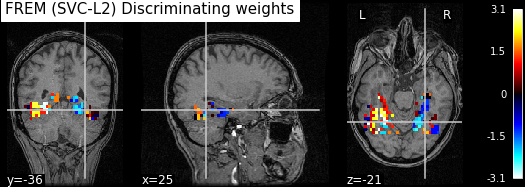
\includegraphics[width=.5\linewidth, height=4cm,  valign=c]{images/FREM (SVC-L2) Discriminating weights anat.png}
    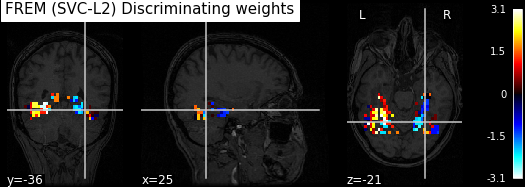
\includegraphics[width=.5\linewidth, height=4cm,  valign=c]{images/FREM (SVC-L2) Discriminating weights.png}
    \\[\smallskipamount]
    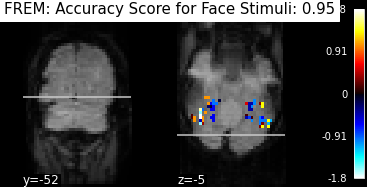
\includegraphics[width=.5\linewidth, height=4cm,  valign=c]{images/FREM_face.png}
    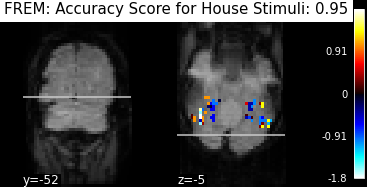
\includegraphics[width=.5\linewidth, height=4cm,  valign=c]{images/FREM_house.png}
    \caption{Visualizations of discriminate power of FREM decoder at first row. In second row, the visuals represent the discrimination of neural responses when face and house stimuli is presented.}\label{fig:frem}
\end{figure*}


\subsection{Classical Machine Learning to Ensemble Robust Decoding}
We applied more than 30 decoding algorithms, here we listed our methods and their brief descriptions.
\subsubsection{LinearSVC}
Support Vector with the linear kernel is an efficient algorithm for linearly separable data spaces by fitting hyper-plane that categorizes the visual stimuli in our context \cite{scikit-learn}. 

\subsubsection{SGD Classifier}
SGD classifier is a linear classifier that use stochastic gradient descent with Hinge loss to separate data spaces. We SGD classifier is implemented with l1 regularization \cite{scikit-learn}. 
\subsubsection{MLP}
MLP is a simple neural network architecture that consists of a bunch of linear layers with ReLU non-linearity, and optimized by the Stochastic Gradient Descent rule \cite{scikit-learn}.

\subsubsection{Perceptron}
Perceptron is a single layer version of MLP and uses log-loss instead of Cross-Entropy \cite{scikit-learn}.

\subsubsection{Logistic Regression}
Logistic regression is a classical machine learning algorithm, it applies linear transformation on the data followed by sigmoidal activation to generate real valued probabilities \cite{scikit-learn}.

\subsubsection{Logistic Regression Cross-Validation}
We also performed 10-Fold cross-validation with logistic regression. It produces more reliable results compared to conventional logistic regression \cite{scikit-learn}. 

\subsubsection{SVC}
Support Vector Classifier is a powerful paradigm in the context of classification. It is classical SVM with radial basis function kernel \cite{scikit-learn}.

\subsubsection{Calibrated Classifier}
It is a cross-validated probability calibration classifier with isotonic logistic regression \cite{scikit-learn}.

\subsubsection{Passive Aggressive Classifier}
Passive Aggressive classifier is margin based online large-scale learning algorithm similar to perceptron but does not require learning rate \cite{crammer2006online, scikit-learn}.

\subsubsection{Label Propagation Classifier}
Label Propagation classifier is semi-supervised graph inference algorithm that iterates on the original graph and normalizes the edge weights by graph Laplacian \cite{heckemann2006automatic, scikit-learn}.

\subsubsection{Random Forest Classifier}
Random Forest classifier is a meta estimator algorithm that fits parallel decision tree classifiers with bootstraped samples of the original dataset to improve the predictive accuracy and model reliability \cite{scikit-learn}.

\subsubsection{Gradient Boosting Classifier}
Gradient boosting classifier is boosting algorithm that ensembles a weak learnings, generally decision trees. It constructs an additive model in a forward stage-wise fashion that enables model to optimize the parameters on any differentiable loss functions. We utilized 100 weak learners to construct end classifier \cite{scikit-learn}. 

\subsubsection{Quadratic Discriminant Classifier}
Quadratic Discriminant classifier is class conditional density algorithm with quadratic decision boundaries to fit seperate Gaussian to each classes. It is a powerful method when we have priory knowledge that individual classes exhibit distinct covariance \cite{scikit-learn}.

\subsubsection{Ridge Classifier}
Ridge classifier is L2 penalized version of logistic regression that helps robust decoding with lower degrees of freedom \cite{scikit-learn}.


\begin{table*}[]
\noindent
\centering
\begin{tabular}{l|llll}
Model                  & \multicolumn{1}{l|}{Accuracy}            & \multicolumn{1}{l|}{Balanced Accuracy}    & \multicolumn{1}{l|}{F1 Score}             & Time Taken (sec)           \\ \hline
\textbf{FREM:LR-L2} &
  \multicolumn{1}{l|}{0.95} &
  \multicolumn{1}{l|}{0.96} &
  \multicolumn{1}{l|}{0.94} &
  - \\
\textbf{FREM:SVC-L2} &
  \multicolumn{1}{l|}{0.94} &
  \multicolumn{1}{l|}{0.94} &
  \multicolumn{1}{l|}{0.94} &
  - \\
CalibratedClassifierCV &
  \multicolumn{1}{l|}{0.87} &
  \multicolumn{1}{l|}{0.88} &
  \multicolumn{1}{l|}{0.87} &
  2.78 \\
PassiveAggressiveClassifier &
  \multicolumn{1}{l|}{0.86} &
  \multicolumn{1}{l|}{0.86} &
  \multicolumn{1}{l|}{0.86} &
  1.55 \\
LogisticRegression &
  \multicolumn{1}{l|}{0.85} &
  \multicolumn{1}{l|}{0.85} &
  \multicolumn{1}{l|}{0.85} &
  0.64 \\
RidgeClassifierCV &
  \multicolumn{1}{l|}{0.85} &
  \multicolumn{1}{l|}{0.85} &
  \multicolumn{1}{l|}{0.85} &
  2.14 \\
LinearSVC &
  \multicolumn{1}{l|}{0.84} &
  \multicolumn{1}{l|}{0.84} &
  \multicolumn{1}{l|}{0.84} &
  0.49 \\
Perceptron &
  \multicolumn{1}{l|}{0.83} &
  \multicolumn{1}{l|}{0.83} &
  \multicolumn{1}{l|}{0.83} &
  0.67 \\
Twin-SVT &
  \multicolumn{1}{l|}{0.82} &
  \multicolumn{1}{l|}{-} &
  \multicolumn{1}{l|}{-} &
  - \\
LinearDiscriminantAnalysis &
  \multicolumn{1}{l|}{0.81} &
  \multicolumn{1}{l|}{0.81} &
  \multicolumn{1}{l|}{0.81} &
  0.23 \\
3D CNN &
  \multicolumn{1}{l|}{0.8} &
  \multicolumn{1}{l|}{-} &
  \multicolumn{1}{l|}{-} &
  - \\
SGDClassifier &
  \multicolumn{1}{l|}{0.79} &
  \multicolumn{1}{l|}{0.79} &
  \multicolumn{1}{l|}{0.79} &
  0.26 \\
NuSVC &
  \multicolumn{1}{l|}{0.75} &
  \multicolumn{1}{l|}{0.761} &
  \multicolumn{1}{l|}{0.75} &
  0.53 \\
RidgeClassifier &
  \multicolumn{1}{l|}{0.74} &
  \multicolumn{1}{l|}{0.74} &
  \multicolumn{1}{l|}{0.74} &
  1.23 \\
SVC &
  \multicolumn{1}{l|}{0.73} &
  \multicolumn{1}{l|}{0.74} &
  \multicolumn{1}{l|}{0.73} &
  0.42 \\
LGBMClassifier &
  \multicolumn{1}{l|}{0.71} &
  \multicolumn{1}{l|}{0.72} &
  \multicolumn{1}{l|}{0.71} &
  5.62 \\
XGBClassifier &
  \multicolumn{1}{l|}{0.70} &
  \multicolumn{1}{l|}{0.71} &
  \multicolumn{1}{l|}{0.70} &
  6.32 \\
2D CNN &
  \multicolumn{1}{l|}{0.7} &
  \multicolumn{1}{l|}{-} &
  \multicolumn{1}{l|}{-} &
  - \\
RandomForestClassifier &
  \multicolumn{1}{l|}{0.69} &
  \multicolumn{1}{l|}{0.69} &
  \multicolumn{1}{l|}{0.69} &
  6.60 \\
ExtraTreesClassifier &
  \multicolumn{1}{l|}{0.66} &
  \multicolumn{1}{l|}{0.67} &
  \multicolumn{1}{l|}{0.66} &
  3.47 \\
KNeighborsClassifier &
  \multicolumn{1}{l|}{0.60} &
  \multicolumn{1}{l|}{0.61} &
  \multicolumn{1}{l|}{0.60} &
  0.47 \\
BaggingClassifier &
  \multicolumn{1}{l|}{0.50} &
  \multicolumn{1}{l|}{0.50} &
  \multicolumn{1}{l|}{0.49} &
  0.96 \\
NearestCentroid &
  \multicolumn{1}{l|}{0.39} &
  \multicolumn{1}{l|}{0.40} &
  \multicolumn{1}{l|}{0.40} &
  0.17 \\
DecisionTreeClassifier &
  \multicolumn{1}{l|}{0.37} &
  \multicolumn{1}{l|}{0.38} &
  \multicolumn{1}{l|}{0.38} &
  0.07 \\
BernoulliNB &
  \multicolumn{1}{l|}{0.36} &
  \multicolumn{1}{l|}{0.36} &
  \multicolumn{1}{l|}{0.35} &
  0.08 \\
GaussianNB &
  \multicolumn{1}{l|}{0.35} &
  \multicolumn{1}{l|}{0.35} &
  \multicolumn{1}{l|}{0.34} &
  0.05 \\
ExtraTreeClassifier &
  \multicolumn{1}{l|}{0.30} &
  \multicolumn{1}{l|}{0.31} &
  \multicolumn{1}{l|}{0.29} &
  0.04 \\
AdaBoostClassifier &
  \multicolumn{1}{l|}{0.24} &
  \multicolumn{1}{l|}{0.25} &
  \multicolumn{1}{l|}{0.21} &
  1.41 \\
QuadraticDiscriminantAnalysis &
  \multicolumn{1}{l|}{0.15} &
  \multicolumn{1}{l|}{0.16} &
  \multicolumn{1}{l|}{0.15} &
  0.17 \\
LabelPropagation &
  \multicolumn{1}{l|}{0.14} &
  \multicolumn{1}{l|}{0.12} &
  \multicolumn{1}{l|}{0.03} &
  0.08 
\end{tabular}
\caption{\label{tab:results} \textbf{fMRI Decoding Accuracy Scores}. Decoding winner is FREM algorithm with Logistic Regression. Deep learning based methods could not outperform the ensemble ones since classical ML algorithms performed on the masked ventral temporal cortex region whereas DL algorithms performed in whole brain area of interest. Best results are bolded.}
\end{table*}



\subsubsection{Ridge Classifier Cross-Validation}
Ridge classifier cross-validation is more reliable version of Ridge Classifier by estimating its model parameters by 10-Fold cross validation \cite{scikit-learn}.

\subsubsection{AdaBoost Classifier}
AdaBoost classifier is type of ensemble learning algorithm that fits weak classifier on the dataset then fits additional copies of the classifier with adjusted parameters based on the incorrectly classified objects \cite{scikit-learn}.

\subsubsection{Extra Trees Classifier}
Extra Trees classifier is another ensemble learning method based on randomized decision trees on the sub-sampled version of the datasets to improve predictive quality \cite{scikit-learn}.

\subsubsection{K-Neighbors Classifier}
K-Neighbors classifier is an instance-based learning method based on $k$ neighbors to consider. We consider 5 neighbors with minkowski distance metric to vote class predictions \cite{scikit-learn}.

\subsubsection{Bernoulli Naive Bayes Classifier}
Bernoulli Naive Bayes classifier applies Bayesian rule to dataset with prior assumption that the data comes form multivariate Bernoulli distribution \cite{scikit-learn}.

\subsubsection{Gaussian Naive Bayes Classifier}
Gaussian Naive Bayes classifier applies Bayesian rule to dataset with prior assumption that the data comes form multivariate Gaussian distribution \cite{scikit-learn}.

\subsubsection{Nu-Support Vector Classifier}
Nu-Support Vector classifier is type of SVM algorithm. It is very similar to SVC but it differs from its controllability of a number of support vectors \cite{scikit-learn}.

\subsubsection{Nearest Centroid Classifier}
In Nearest Centroid classifier, each class is represented by with class centroid. New samples are classified based on the distance to class centroid, so it is very similar to the supervised version of K-means \cite{scikit-learn}.

\subsubsection{Bagging Classifier}
Bagging classifier is an ensemble learning method that fits base classifiers to random subsets of the original dataset. Then, the predictions are aggregated either by voting or averaging to produce end class-wise predictions \cite{scikit-learn}.

\subsubsection{FREM: Cross-Validated Ensemble of L2 regularized SVCs and Logistic Regressions}
FREM uses an implicit spatial regularization through fast clustering and aggregates a high number of estimators trained on various splits of the training set, thus returning a very robust decoder at a lower computational cost than other spatially regularized methods \cite{sklearn_api} that improve decoding accuracy with lower degree of computation. We both construct FREM based on SVCs and Logistic Regression units \cite{sklearn_api}. 


\subsection{Convolutional Neural Networks to Vision Transformers}
We further performed deep learning algorithms from CNNs to vision transformers. All models are optimized with Cross Entropy loss, Adam optimizer with starting learning rate as 1e-3. Scheduled learning rate scaler is performed to decrease the learning rate by \% 80 at every epoch. Batch size is varied from 16 to 64. One single Tesla K80 GPU is used for all experiments. Architecture details and their visuals of both CNNs and vision transformer are depicted in appendix \ref{appendix:C}, \ref{appendix:D} and \ref{appendix:E}, respectively. Please refer for further information. All deep learning algorithm are performed in the whole brain area represented as fMRI form instead of RoI's of subjects.

\subsection{2D CNN}
We developed 2D CNN architecture to decode fMRI samples. In the architecture, there are 4 special convolutional blocks, each block is consists of a sequel of Convolution, Batch Normalization, ReLU, Max Pooling and Dropout layer. To classify, the representative feature vector is propagated to linear blocks. There are two linear blocks, each block consist of sequel of linear layer, batch normalization, ReLU and dropout layer. We provide details of the architecture in appendix \ref{appendix:C}.

\subsection{3D CNN}
3D CNN is developed to perform spatio-temporal decoding of fMRI's of whole brain region. The architecture is nearly the same as the 2D case except all layers are 3D, i.e., 2D convolutions are interchanged with 3D's, then Batch Normalization, Max Pooling and Dropout layers are now extended to 3D case. We provide details of the architecture and its visualization in appendix \ref{appendix:D}.

\subsection{Vision Transformers}
Vision transformers are recently proposed paradigm that replaced with CNN blocks with multi-head self attention mechanism. As vision transformer, we performed experiments in twin-svt \cite{chu2021twins} that is state-of-the-art vision transformer with its unique attention mechanism called spatially separable self-attention (SSSA) module SSSA module consists of spatially oriented both global and local attention mechanism by taking the advantage of interactions between different streams of visual representations. We provide details of the transformer in appendix \ref{appendix:E}. We highly recommend reader to refer to appendix \ref{appendix:E} for a detailed understanding of twin-svt.    

\section{Results}
Decoding results are presented in table \ref{tab:results}. Winner brain decoder is FREM based methods. FREM is a powerful paradigm in the context of brain decoding since it aggregates similar voxels together to reduce the dimensionality of the RoI of subjects with an ensemble of different methods. It is highly spatially regularized method and combines high number of parallel estimators trained on different sub-spaces of the original data. We visualized discriminate weights of FREMs on fMRI images with corresponding RoIs of subjects in figure \ref{fig:frem} at the top row. Further, we visualized the decoding accuracy of FREMs when face and house stimuli is presented figure \ref{fig:frem} at bottom row. When visuals of faces and houses are presented to the subjects, FREMs perform better with respect to other stimulus types. Then, Calibrated classifier is placed as third among decoders by achieving \% 87 accuracy. Then, Passive Aggressive classifier and Logistic Regression are also performed quite well in brain decoding. In terms of deep learning methods, twin transformed outperforms both 2D and 3D CNNs by a considerable margin thanks to its spatially oriented self-separable attention mechanism. Another big plus of the transformer is that it is far away explainable than any DL based approaches that will quite an important step in further discovery of attention mechanism, especially covert attention, in human brains. It may demonstrate interactions of important regions of spatial connections of human brain that play a significant role in spatio-temporal decoding. 

\section{Discussion}
Our experiments are motivated by addressing the issue of whether patterns of neural responses recorded by fMRI when visuals stimuli is presented are discriminate or not. This paper addresses the advances of understanding in distributed and overlapping patterns of neural activity to infer the functional role of brain areas and networks. To expose that, we performed functional connectivity and similarity analysis, and concluded that responses evoked in RoIs of the ventral temporal cortex are highly correlated with all measures except for partial correlation. Partial correlation is relatively less in that regions. Then, we performed a bunch of dimension reduction and manifold learning algorithm to visualize the underlying geodesic manifolds of the regions. All methods except for LDA demonstrate that there are highly overlapping and distributed representations in that areas. However, LDA show that even there are highly correlated and overlapping responses, we can discriminate them by powerful decoding algorithms. Further, we run more than 30 different fMRI decoding algorithm on the ventral temporal masked regions, and conclude that state-of-the-art robust decoding algorithm FREM with either SVCs and Logistic Regression, outperforms all both ML and DL based methods as it achieves more than \% 95 accuracy. The reason behind the deep learning based methods, i.e., 2D-3D CNNs and vision transformers, could not outperform the ML based ones is that ML decoders are performed on the ventral temporal masked regions of the subjects whereas DL decoders are performed in whole brain areas. However, the vision transformer outperformed other DL decoders and demonstrate the power of spatially oriented attention mechanism that mimics the human attention mechanism in deeper way. To our best knowledge, we either achieved either competitive accuracy on current state-of-the-art or outperformed by a small margin \cite{treder2020mvpa, norman2006beyond}. We further demonstrate that with the spatially oriented vision transformers that expose both global and local attention in distributed regions in the brain, we explain and enlight the covert attention mechanisms in the human brain by its encoded neural response, as it achieves \% 82 accuracy even the algorithm scans the whole brain region. Further research along with the decoding of brain by spatially oriented vision transformers can expose the underlying reasons regarding the why, when and how human attention mechanism is oriented in a computational manner. We further conclude that multi-voxel pattern recognition methods with cutting-edge techniques, e.g., vision transformers, may advance our understanding of neural information processing and neural coding from visual perception to memory search. Code is available at appendix \ref{appendix:F}.     



%\cite{wang2021endtoend}
%\cite{hu2019learning}
%\cite{bertasius2020classifying}
%\newpage
%------------------------------------------------------------------------


{\small
\bibliographystyle{ieee}
\bibliography{egbib}
}

%\clearpage
\appendix 
\section{Samples of Visual Stimuli}
\label{appendix:A}
Example of stimuli are presented in figure \ref{fig:stimuli}.

\begin{figure*}
\centering
     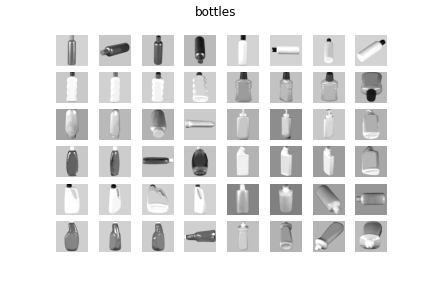
\includegraphics[width=.33\linewidth, height=3cm,  valign=c]{images/bottles.png}
    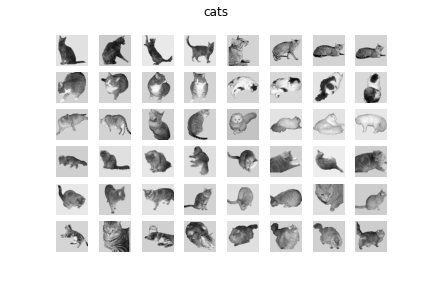
\includegraphics[width=.33\linewidth, height=3cm,  valign=c]{images/cats.png}
    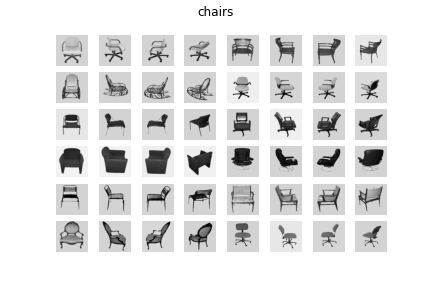
\includegraphics[width=.33\linewidth, height=3cm,  valign=c]{images/chairs.png}
    \\[\smallskipamount]
    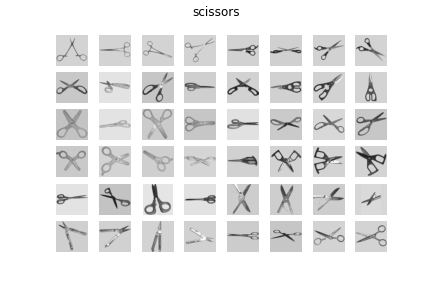
\includegraphics[width=.33\linewidth, height=3cm,  valign=c]{images/scissors.png}
    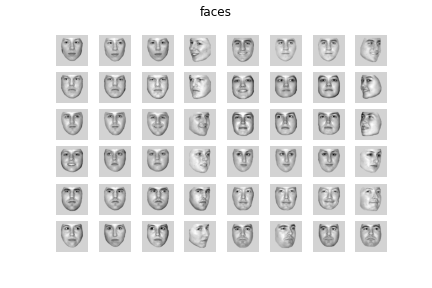
\includegraphics[width=.33\linewidth, height=3cm,  valign=c]{images/faces.png}
    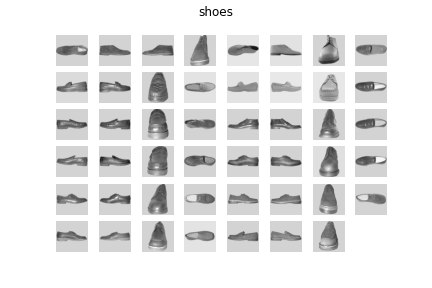
\includegraphics[width=.33\linewidth, height=3cm,  valign=c]{images/shoes.png}
    \caption{Examples of stimuli visuals. They are gray scale images from different kind of nature.
}\label{fig:stimuli}
\end{figure*}


\section{Echo-Planar Imaging for 4D Visualization of the fMRI}
\label{appendix:B}
Echo-planar, temporally averaged fMRI visualization is presented at figure \ref{fig:epi}
\begin{figure*}
\begin{center}
 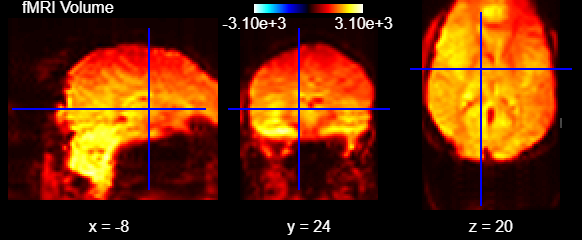
\includegraphics[width=1\linewidth]{images/indir.png}
\end{center}
   \caption{Echo-Planar Imaging for 4D Visualization of the fMRI on subject, averaged for 4D}
\label{fig:epi}
\end{figure*}


\section{2D CNN Details}
\label{appendix:C}
Detailed architecture of 2D CNN is depicted in figure \ref{fig:2dcnn}.

\begin{figure*}
\centering
 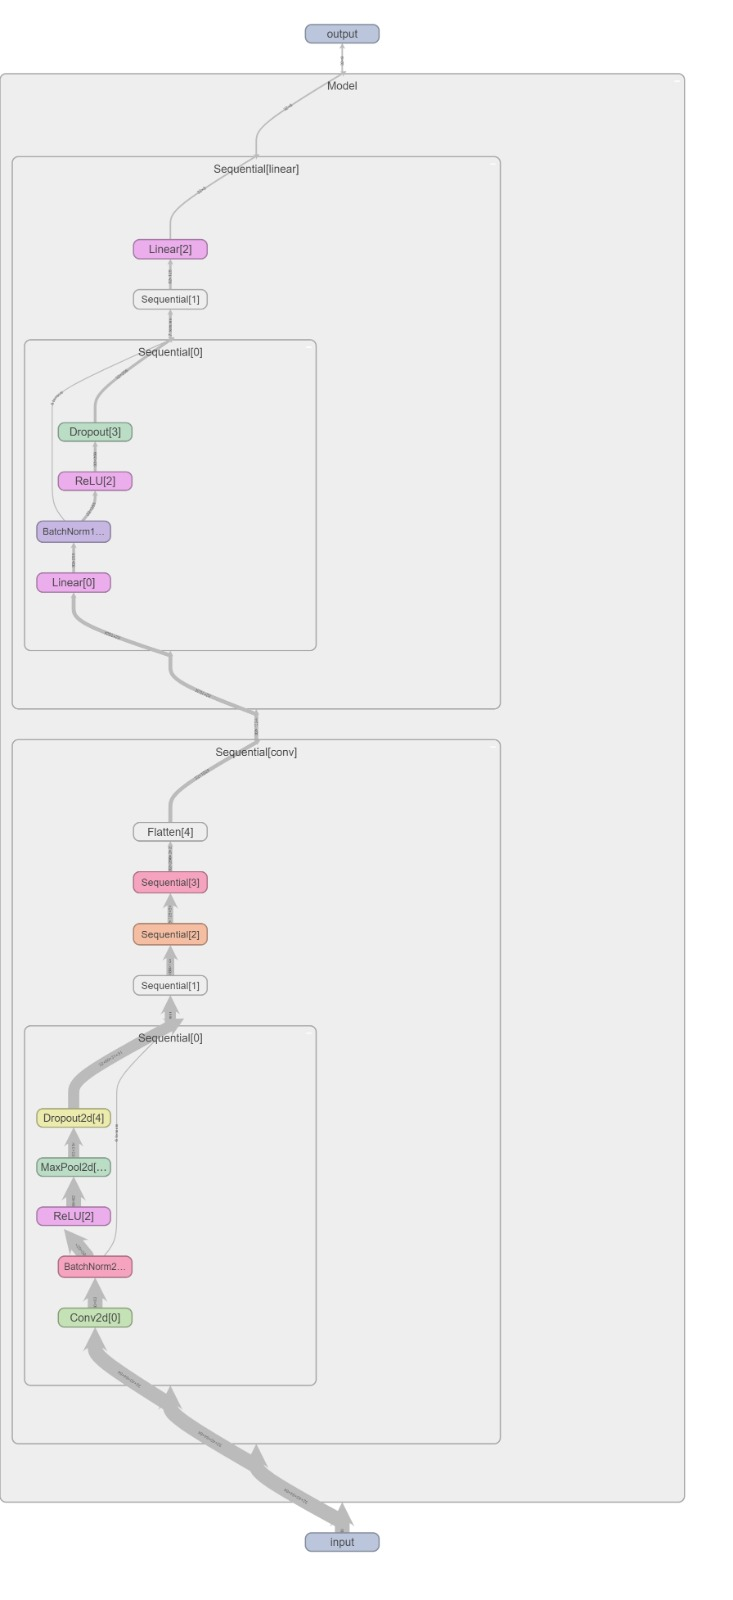
\includegraphics[width=0.8\linewidth, height = 21cm]{images/2dcnn.jpeg}
   \caption{\textbf{Architecture of 2D CNN}. In the architecture, there are 4 special convolutional blocks, each block is consist of sequel of Convolution, Batch Normalization, ReLU, Max Pooling and dropout layer. To classify, the representative feature vector is propagated to linear blocks. There are two linear blocks, each block consist of sequel of linear layer, batch normalization, ReLU and dropout layer.}
\label{fig:2dcnn}
\end{figure*}

\section{3D CNN Details}
\label{appendix:D}
Detailed architecture of 3D CNN is depicted in figure \ref{fig:3dcnn}.
\begin{figure*}
\centering
 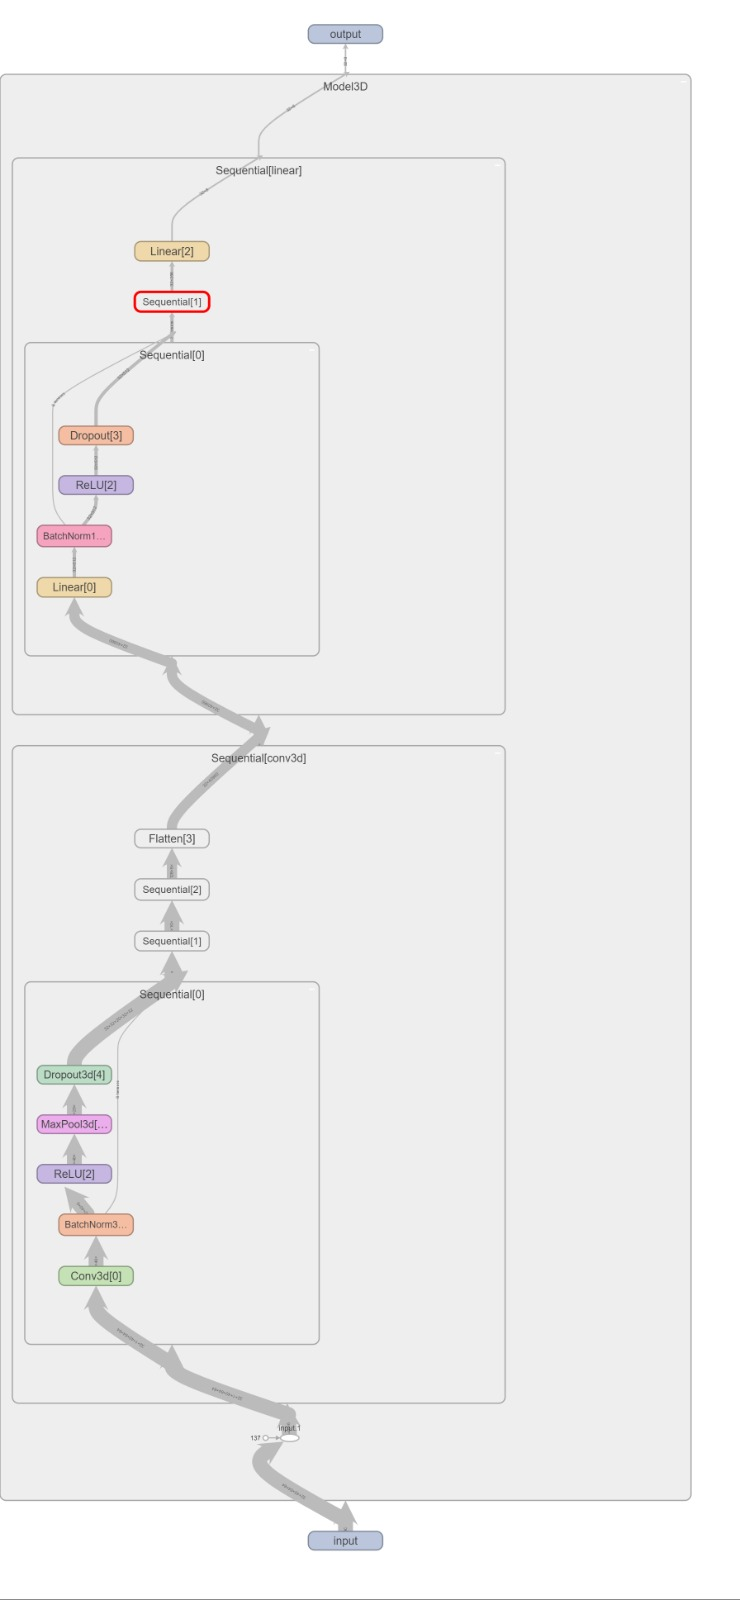
\includegraphics[width=0.8\linewidth, height = 21cm]{images/3dcnn.jpeg}
   \caption{\textbf{Architecture of 3D CNN}. In the architecture, there are 4 special convolutional blocks, each block is consist of sequel of Convolution, Batch Normalization, ReLU, Max Pooling and dropout layer in 3D. To classify, the representative feature vector is propagated to linear blocks. There are two linear blocks, each block consist of sequel of linear layer, batch normalization, ReLU and dropout layer in 3D.}
\label{fig:3dcnn}
\end{figure*}

\begin{figure*}
\centering
 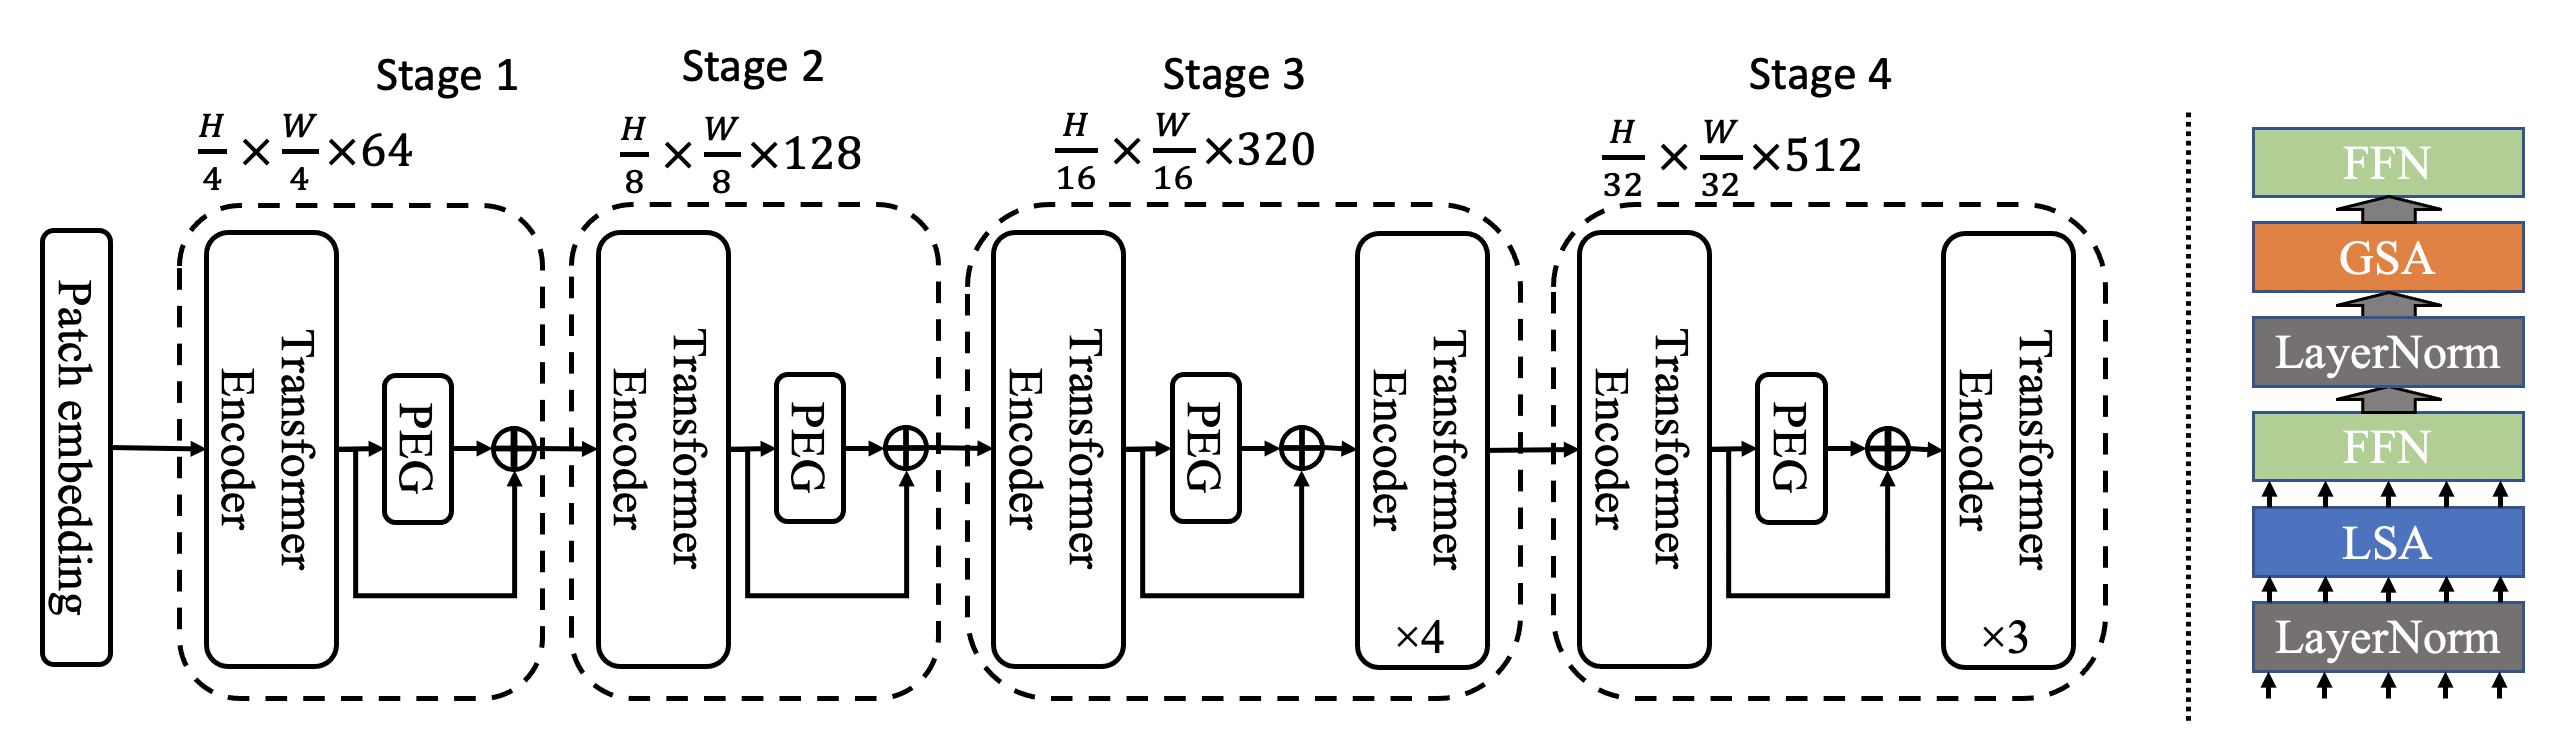
\includegraphics[width=1\linewidth]{images/tt.png}
   \caption{\textbf{Architecture of Twin Transformer}. Given the input, Twins-SVT interleaves locally-grouped attention (LSA) and global sub-sampled attention (GSA) in hierarchical stages. PEG stands for position encoding generator.}
\label{fig:twins}
\end{figure*}

\section{Twin Transformer Details}
\label{appendix:E}
Recently, twins are proposed in the paper \cite{chu2021twins}, and demonstrate that the spatially oriented vision transformers can outperform the classical CNNs \cite{chu2021twins}. Here, we integrated Twins-SVT network to our case to produce high qualtiy decoding. There twin transformer is based on a spatially separable self-attention (SSSA) network that consist of locally-grouped self-attention (LSA) and global sub-sampled attention (GSA) \cite{chu2021twins}. Thanks to its spatially separable module, the quality of features are increased by a significant margin. In the subsections, we describe the SSSA module in detail.  



\subsection{Locally-grouped self-attention (LSA)}
In LSA, 2-D feature maps are divided into sub-windows that enable the self-attention within each sub-window. Features maps are divided into $m$ x $n$ sub-windows, that lead to each window consist of $\frac{HW}{mn}$ elements where H,W represents image dimensions. By dividing the image into $m$ x $n$ region the computational cost is decreased from $ O(H^2W^2d)$ to $O(\frac{H^2W^2}{mn}d)$ where d is the self-attention dimension. At that point, we did not make any further relation to non-overlapping regions in the windows. Hence, here GSA module comes into play.



\subsection{Global sub-sampled attention (GSA)}
As we need further localization in the self-attention mechanism, global self-attention is required to make connections in non-overlapping regions. In GSA module, a single representative key in formations from the locally attended windows are used to compute global attention. However, with the computation of global-attention, the computation cost would increase to $ O(H^2W^2d)$. To prevent this, locally attended features are sub-sampled via average pooling, depth-wise strided convolutions and regular strided convolutions. The results show that regular strided convolutions perform best \cite{chu2021twins}. Mathematically, SSSA module performs the following computations.

\begin{align}
\label{eqn:eqlabel}
\begin{aligned}
     a_{i,j}^l &= LSA(LayerNorm(a_{i,j}^{l-1})) + a_{i,j}^{l-1},
    \\
     a_{i,j}^l &= FFN(LayerNorm(a_{i,j}^{l})) + a_{i,j}^{l},
    \\
     a^{l+1} &= GSA(LayerNorm(a^{l})) + a^{l},
    \\
    a^{l+1} &= FFN(LayerNorm(a^{l + 1})) + a^{l+1} 
\end{aligned}
\end{align}
for $i = 1,...,m$ and $j = 1,...n$ where LSA denotes locally-grouped self-attention, GSA denotes global sub-sampled attention, FFN denotes feed-forward network and LayerNorm denotes layer normalization layer \cite{ba2016layer}. %Both attention modules performed in multi-headed way.

\clearpage
\onecolumn
\section{Code}
\label{appendix:F}

\begin{lstlisting}[language=Python]
#!/usr/bin/env python
# coding: utf-8

# #                        - Computational Neuroscience 2021-2022 Final Project -        

# ##   Project Name: Combinatorial Codes in Ventral Temporal Lobe for Visual Object Recognition
# 
# 

# Filename       : CompNeuro_2021-2022_Final_Project.ipynb
# 
# Authors        : Can Kocagil, Emirhan Ilhan and Arman Vural Budunoglu, 
# 
# Institution    : Bilkent University Departman of Electric & Electronical Enginering
# 
# Class          : EEE482/582 - Computational Neuroscience 
# 
# Project Goal   : Implement multi-voxel pattern analyses methods (based on some type of classifier) to
#                  decode the category of visual stimuli viewed by a human subject based on their recorded brain activity
#                  
# Dataset Link   : https://openfmri.org/dataset/ds000105.
# 
# Related Papers : Distributed and overlapping representations of faces and objects in ventral temporal cortex

# Pipeline:
#     
#     1) Necessary Installations (If necessary)
#     2) Imports
#     3) Visual Stimuli and Category Loading
#     4) Visual Stimuli Transformations
#     5) Explanatory Visual Stimuli Analysis
#         
#         * PCA
#         * T-Stochastic Neighboor Embedding (t-SNE)
#         * Linear Discriminate Analysis
#         * Uniform Manifold Approximation and Projection (UMAP)
#         * Independent Component Analysis (ICA)
#         * Non-Negative Matrix Factorization
#         * Masking
#         
#     6) Visual Stimuli Similarity Analysis
#     
#         * Euclidean Similarity
#         * Cosine Similarity
#         * Pearson Correlation             
#         
#     7) Classical ML Algorithms:
#     
#         * LinearSVC
#         * SGDClassifier
#         * MLPClassifier
#         * Perceptron
#         * LogisticRegression
#         * LogisticRegressionCV
#         * SVC
#         * CalibratedClassifierCV
#         * PassiveAggressiveClassifier
#         * LabelPropagation
#         * LabelSpreading
#         * RandomForestClassifier
#         * GradientBoostingClassifier
#         * QuadraticDiscriminantAnalysis
#         * RidgeClassifierCV
#         * RidgeClassifier
#         * AdaBoostClassifier
#         * ExtraTreesClassifier
#         * KNeighborsClassifier
#         * BaggingClassifier
#         * BernoulliNB
#         * LinearDiscriminantAnalysis
#         * GaussianNB
#         * NuSVC
#         * DecisionTreeClassifier
#         * NearestCentroid
#         * ExtraTreeClassifier
#         * CheckingClassifier
#         * DummyClassifier
#         
#     7) Reported Metrics
#         * Accuracy
#         * Balanced Accuracy
#         * ROC AUC
#         * F1-Score
#         * Time Taken
#         
#     8) Deep Learning Algorithms
#         * 3-D Convolutional Neural Networks
#         * Visual Transformers
#         * ...
#         
#     9) Results Interpretation
#     
# 
# 
# 
# 

# # Necessary Installations (If necessary)

# In[1]:


get_ipython().system('pip install umap')
get_ipython().system('pip install pipreqs')
get_ipython().system('pip install lazypredict')
get_ipython().system('pip install nibabel')
get_ipython().system('pip install nilearn')
get_ipython().system('pip install -U kaleido')


try:
    import sklearn
    print('Scikit-learn is available, version', sklearn.__version__)
    
except:
    get_ipython().system('pip install scikit-learn')
    
 
try:
    import cv2
    print('Open-CV is available, version', cv2.__version__)
    
except:
     get_ipython().system('pip install opencv-python')
    
   
try:
    import seaborn
    print('Seaborn is available, version', seaborn.__version__)
    
except:
     get_ipython().system('pip install seaborn')


# # Imports

# In[1]:


from __future__ import print_function, division

# Basics:
import numpy as np,pandas as pd, matplotlib.pyplot as plt, seaborn as sns
import os, random, time, sys, copy, math, pickle

# interactive mode
plt.ion()

# Ignore warnings
import warnings
warnings.filterwarnings("ignore")

# For plotting
import plotly.io as plt_io
import plotly.graph_objects as go
get_ipython().run_line_magic('matplotlib', 'inline')

# Dimension Reduction Algorithms:
from sklearn.decomposition import PCA
from sklearn.manifold import TSNE
from sklearn.discriminant_analysis import LinearDiscriminantAnalysis as LDA
from sklearn.decomposition import FastICA
from sklearn.decomposition import NMF
import umap

# Transformations
from sklearn.preprocessing import StandardScaler
from sklearn.preprocessing import MinMaxScaler

# Metrics:
from sklearn.metrics import classification_report

# Train-Test Splitter:
from sklearn.model_selection import train_test_split

# For Classical ML algorithms:
from lazypredict.Supervised import LazyClassifier

# Utilies:
from tqdm import tqdm

# For distance measurements:
from scipy.spatial.distance import cdist

# Extras:
from abc import abstractmethod
from typing import Callable, Iterable, List, Tuple

# Set true for Google Colab:
COLAB = False

if COLAB:
    # To access Google Drive:
    from google.colab import drive
    drive.mount("/content/gdrive")

    
# For neuroimaging:
from nibabel.testing import data_path
from nilearn import plotting as nplt
from nilearn.input_data import NiftiMasker
from nilearn import datasets
from nilearn import plotting
from nilearn.image import mean_img
from nilearn.image import index_img
import nibabel as nib
from nilearn import image



print("NumPy Version: ", np.__version__)


root_dir = os.getcwd()
image_results_dir = os.path.join(root_dir, 'images')
results_dir = os.path.join(root_dir, 'results')

print('Working Directory: \n ', root_dir)


# Creating requirements.txt file
get_ipython().system('pip3 freeze > requirements.txt  ')


# # Utilities

# In[2]:


from utils.timers import timeit
from utils.metrics import accuracy, confusion_matrix, visualize_confusion_matrix
from utils.savers import save, save_obj, load, load_obj
from utils.reproduce import random_seed
from dataset.fetch_data_matrix import fetch_from_haxby
from visualizer.plot2D import plot_2d
from visualizer.plot3D import plot_3d  




# In[3]:


# There are 6 number of subjects in the experiment: 
haxby_dataset = datasets.fetch_haxby(subjects= [1,2,3,4,5,6])


# In[4]:


haxby_dataset


# In[5]:


num_subjects = 6

for subject in range(num_subjects):   

    # 'func' is a list of filenames: one for each subject
    fmri_filename = haxby_dataset.func[subject]

    # print basic information on the dataset
    print('First subject functional nifti images (4D) are at: %s' %
          fmri_filename)  # 4D data


# # Explanatory Visual Stimuli Analysis

# ## Echo-planar imaging (EPI) Averaging for 4-D Visualization of the fMRI Nifti Image

# In[7]:


explanatory_fMRI_dir = os.path.join(image_results_dir, 'explanatory')

# cut in x-direction
sagittal = -25
# cut in y-direction
coronal = -37
# cut in z-direction
axial = -6

# coordinates displaying should be prepared as a list
cut_coords = [sagittal, coronal, axial]


# Echo-planar imaging (EPI) Averaged for 4-D
epi_image = mean_img(fmri_filename)

plotting.view_img(epi_image,
                  threshold=None,
                  title = 'fMRI Volume',
                  output_file = os.path.join(explanatory_fMRI_dir + 'fMRI_volume.png'),
                  )


# ## A mask of the Ventral Temporal (VT) cortex with egion of Interest (RoI) 

# In[14]:


from visualizer.roi import RoI_visualizer


# In[15]:


RoI_visualizer(haxby_dataset, subject_id=2)


# ## Statistical Maps

# In[16]:


subject_id =  3

plotting.plot_stat_map(mean_img(fmri_filename),
                       threshold=3,
                       figure=plt.figure(figsize=(12,4)),
                       title=f'Statistical Map of fMRI images of subject {subject_id}',
                       #output_file = os.path.join(explanatory_fMRI_dir, 'stats_map.png')
                       )
plt.show()


# ## Simple, Compact, fMRI Visualizations 

# In[27]:


plotting.plot_img(mean_img(fmri_filename),
                 cut_coords=None,
                 #output_file= os.path.join(explanatory_fMRI_dir, 'fMRI.png'),
                 display_mode='ortho',
                 figure=plt.figure(figsize = (12,4)),
                 axes=None,
                 title='Visualization of fMRI Data',
                 threshold=3,
                 annotate=True,
                 draw_cross=True,
                 black_bg=False,
                 colorbar=False)
plt.show()


# ## EPI Plotting 

# In[28]:


plotting.plot_epi(mean_img(fmri_filename),
                  title='Smoothed mean EPI',
                  cut_coords=cut_coords,
                  #output_file= os.path.join(explanatory_fMRI_dir, 'epi.png')
                 )


# ## Anatomic fMRI Visualizations

# In[31]:


plotting.plot_anat(haxby_dataset.anat[0],
                  cut_coords=cut_coords,
                  #output_file= os.path.join(explanatory_fMRI_dir, 'anat.png'),
                  display_mode='ortho',
                  figure=plt.figure(figsize = (12,4)),
                  axes=None,
                 title='Visualization of fMRI Data',
                 threshold=None,
                 annotate=True,
                 draw_cross=True,
                 black_bg=False,
                 colorbar=False)
plotting.show()


# In[ ]:


plotting.plot_anat(mean_img(fmri_filename),
                  cut_coords=None,
                  output_file=None,
                  display_mode='ortho',
                  figure=plt.figure(figsize = (12,4)),
                  axes=None,
                  title='Visualization of fMRI Data',
                  threshold=None,
                  annotate=True,
                  draw_cross=True,
                  black_bg=False,
                  colorbar=False)
plotting.show()


# ## Plot Haxby masks 

# In[33]:


# Build the mean image because we have no anatomic data


func_filename = haxby_dataset.func[0]
_mean_img = image.mean_img(func_filename)

z_slice = -14

fig = plt.figure(figsize=(4, 5.4), facecolor='k')

from nilearn.plotting import plot_anat, show

display = plot_anat(_mean_img, display_mode='z', cut_coords=[z_slice],
                    figure=fig)

mask_vt_filename = haxby_dataset.mask_vt[0]
mask_house_filename = haxby_dataset.mask_house[0]
mask_face_filename = haxby_dataset.mask_face[0]

display.add_contours(mask_vt_filename,
                     contours=1,
                     antialiased=False,
                     linewidths=4.,
                     levels=[0],
                     colors=['red'])
display.add_contours(mask_house_filename,
                     contours=1,
                     antialiased=False,
                     linewidths=4.,
                     levels=[0],
                     colors=['blue'])
display.add_contours(mask_face_filename,
                     contours=1,
                     antialiased=False,
                     linewidths=4.,
                     levels=[0],
                     colors=['limegreen'])

# We generate a legend using the trick described on
# http://matplotlib.sourceforge.net/users/legend_guide.httpml#using-proxy-artist
from matplotlib.patches import Rectangle
p_v = Rectangle((0, 0), 1, 1, fc="red")
p_h = Rectangle((0, 0), 1, 1, fc="blue")
p_f = Rectangle((0, 0), 1, 1, fc="limegreen")
plt.legend([p_v, p_h, p_f], ["vt", "house", "face"])

plt.show()



#display.savefig(os.path.join(explanatory_fMRI_dir, 'pretty_brain_response.png'))


# ## Glass Brain Plotting 

# In[35]:


plotting.plot_glass_brain(mean_img(fmri_filename),
                          threshold=3,
                          #output_file= os.path.join(explanatory_fMRI_dir, 'glass_brain_white.png')
                          )
plotting.show()


# In[37]:


plotting.plot_glass_brain(
    mean_img(fmri_filename),
    black_bg=True,
    display_mode='xz',
    threshold=None,
    #output_file= os.path.join(explanatory_fMRI_dir, 'glass_brain_black.png')
   )

plotting.show()


# ## Stimuli Visualizations 

# In[38]:


haxby_dataset_stimuli = datasets.fetch_haxby(subjects=[], fetch_stimuli=True)
stimulus_information = haxby_dataset_stimuli.stimuli

for stimulus_type in [*stimulus_information]:
    
    if stimulus_type != 'controls':

        img_paths = stimulus_information[stimulus_type]
        
        fig, axes = plt.subplots(6, 8)
        fig.suptitle(stimulus_type)

        for img_path, ax in zip(img_paths, axes.ravel()):
            image = plt.imread(img_path)
            ax.imshow(image, cmap='gray')

        for ax in axes.ravel():
            ax.axis("off")
            
            
        #fig.savefig(os.path.join(explanatory_fMRI_dir, f'{stimulus_type}.png')) 

plt.show()
    
    


# # Interactive Brain Visualizations 

# ##  3D Plots of statistical maps on the cortical surface

# In[ ]:


plotting.view_img_on_surf(mean_img(fmri_filename), threshold='90%', surf_mesh='fsaverage') 


# In[ ]:


plotting.view_img_on_surf(mean_img(fmri_filename), threshold='70%', surf_mesh='fsaverage') 


# ## Brain Marking

# In[ ]:


plotting.view_markers( 
[(0, -52, 18), (-46, -68, 32), (46, -68, 32), (1, 50, -5)],
['red', 'cyan', 'magenta', 'orange'],
marker_size=10) 


# ## Decoding Label Analysis and Masking 

# In[42]:


# Load behavioral information
behavioral = pd.read_csv(haxby_dataset.session_target[0], delimiter=' ')
behavioral.head()


# In[43]:


# Visual Stimuli Categories:
for stimuli in np.unique(behavioral['labels']).tolist():
    print(stimuli)


# In[6]:


stimuli_categories = [
                        'scissors',
                        'face', 
                        'cat',
                        'scrambledpix',
                        'bottle',
                        'chair',
                        'shoe',
                        'house'
]


# ### Masking Spatio Temporal Code and Its Target 

# In[45]:


# Creating conditional categories:
conditions = behavioral['labels']

# We ignore rest condition:
condition_mask = conditions.isin(stimuli_categories).tolist()


fmri_niimgs = index_img(fmri_filename, condition_mask)

conditions = conditions[condition_mask]

# Convert to numpy array
conditions = conditions.values
print(conditions.shape)


# Spatio-temporal Masked data shape: (temporal dimension, spatial dimension 1, spatial dimension 2, # of experiments)

# In[48]:


# (temporal dimension, spatial dimension 1, spatial dimension 2, # of experiments)
fmri_niimgs.get_data().shape


# Spatio-temporal Un-masked data shape: (temporal dimension, spatial dimension 1, spatial dimension 2, # of experiments)

# In[50]:


spatio_temporal_data = fetch_from_haxby(haxby_dataset.func[subject_id])
spatio_temporal_data.shape


# In[51]:


for subject_id in range(num_subjects):
    label = pd.read_csv(haxby_dataset.session_target[subject_id], delimiter=' ')
    
    # Creating conditional categories:
    conditions = behavioral['labels']

    condition_mask = conditions.isin(stimuli_categories).tolist()
    conditions = conditions[condition_mask]
    
    # Convert to numpy array
    conditions = conditions.values
    print(conditions.shape)   


# # Creatining fMRI Data Matrices for each Subject

# In[7]:


# Creating stimuli to category and category to stimuli:
stimuli2category = {
                        'scissors'     : 0,
                        'face'         : 1, 
                        'cat'          : 2,
                        'scrambledpix' : 3,
                        'bottle'       : 4,
                        'chair'        : 5,
                        'shoe'         : 6,
                        'house'        : 7
}

category2stimuli = {category:stimuli for stimuli, category in stimuli2category.items()}


# ## Spatio-Temporal Masking

# In[8]:


def fetch_haxby_per_subject(subject_id:int = None,standardize:bool = True) -> Tuple[np.ndarray, np.ndarray, np.ndarray]:
    """
    
        Given the subject id, fetch the haxby data in matrix format.
        
        Arguments:
            - subject_id  (int) : Subject number from [1,6]
            - standardize (bool): If true, masks are standardized
            
        Returns:
            - data (Tuple[np.ndarray, np.ndarray, np.ndarray]) = Original 4-D data, Flattened + Masked Data, Label  
    
    """
        
    # Getting the data file name:
    spatio_temporal_data_path = haxby_dataset.func[subject_id]  
   
    # Getting labels:
    behavioral = pd.read_csv(haxby_dataset.session_target[subject_id], delimiter = ' ')
    
    # Creating conditional categories:
    conditions = behavioral['labels']
    
    # Creating masks for stimuli categories, (ignores rest conditions)
    condition_mask = conditions.isin([*stimuli2category]).tolist()
    
    # Appylying masks to labels (categorical):
    conditions = conditions[condition_mask]
    
    # Creating labels series (numerical):
    categories = np.array([stimuli2category[stimulus] for stimulus in conditions])
    
    # Masking fMRI images: (shape = (40, 64, 64, 864))
    fmri_niimgs = index_img(spatio_temporal_data_path, condition_mask)
    
    # Converting NumPy and transposing to (864, 40, 64, 64):
    numpy_fmri = fmri_niimgs.get_data().transpose(3,0,1,2)
    
    masker = NiftiMasker(mask_img=haxby_dataset.mask_vt[subject_id],
                         smoothing_fwhm=4,
                         standardize=standardize,
                         memory='nilearn_cache',
                         memory_level=1)

    masked = masker.fit_transform(fmri_niimgs)
    
    
    return numpy_fmri,  masked, categories


# In[105]:


data = [fetch_haxby_per_subject(subject_id) for subject_id in range(num_subjects)]
fmri_imgs_mat, masks, categories = list(zip(*data))

# Saving the data for future use:
save(fmri_imgs_mat, 'fMRI_data')
save(masks, 'masked_data')
save(categories, 'labels')


# In[102]:


# Loading:
fmri_imgs_mat, masks, categories = load('fMRI_data'), load('masked_data'), load('labels')


# # 4-D fMRI Data Similarity Analysis

# ## Functional Connectivity

# ### Correlation 

# In[59]:


from nilearn.connectome import ConnectivityMeasure
correlation_measure = ConnectivityMeasure(kind='correlation')
correlation_matrix = correlation_measure.fit_transform([masks[subject_id]])[0]

fig = plt.figure()

# Mask out the major diagonal
np.fill_diagonal(correlation_matrix, 0)
plotting.plot_matrix(correlation_matrix,
                     colorbar=True,
                     vmax=0.8, vmin=-0.8,
                     figure = fig)
plotting.show()

fig.savefig(os.path.join(explanatory_fMRI_dir, 'correlation.png'))


# ### Precision 

# In[1]:


correlation_measure = ConnectivityMeasure(kind='precision')
correlation_matrix = correlation_measure.fit_transform([masks[subject_id]])[0]

fig = plt.figure()

# Mask out the major diagonal
np.fill_diagonal(correlation_matrix, 0)
plotting.plot_matrix(correlation_matrix, colorbar=True,
                     vmax=0.8,
                     vmin=-0.8,
                     figure = fig)
plotting.show()


fig.savefig(os.path.join(explanatory_fMRI_dir, 'precision.png'))


# ### Partial Correlation 

# In[62]:


correlation_measure = ConnectivityMeasure(kind='partial correlation')
correlation_matrix = correlation_measure.fit_transform([masks[subject_id]])[0]
fig = plt.figure()

# Mask out the major diagonal
np.fill_diagonal(correlation_matrix, 0)
plotting.plot_matrix(correlation_matrix, colorbar=True,
                     vmax=0.8, vmin=-0.8,figure = fig)
plotting.show()
fig.savefig(os.path.join(explanatory_fMRI_dir, 'partial_correlation.png'))


# ### Cosine 

# In[65]:


fig = plt.figure(figsize=(8,6))
plt.imshow(cdist(masks[subject_id], masks[subject_id], metric='cosine'))
plt.colorbar()
plt.title('Cosine Similarity of Masked fMRI Samples')
plt.show()
fig.savefig(os.path.join(explanatory_fMRI_dir, 'cosine.png'))


# ###  Minkowski

# In[66]:


fig = plt.figure(figsize=(8,6))
plt.imshow(cdist(masks[subject_id], masks[subject_id], metric='minkowski'))
plt.colorbar()
plt.title('Minkowski Similarity of Masked fMRI Samples')
plt.show()
fig.savefig(os.path.join(explanatory_fMRI_dir, 'minkowski.png'))


# ### Euclidean

# In[67]:


fig = plt.figure(figsize=(8,6))
plt.imshow(cdist(masks[subject_id], masks[subject_id]))
plt.colorbar()
plt.title('Euclidean Similarity of Masked fMRI Samples')
plt.show()
fig.savefig(os.path.join(explanatory_fMRI_dir, 'euclidean.png'))


# #  Visual Stimuli Transformations
# 

# In[88]:


# Standardizing the data
scaler = StandardScaler()

# Normalizing data:
minmax_scaler =  MinMaxScaler()


# In[114]:


def plot_2d(component1:np.ndarray, component2:np.ndarray,path:str, y = None, ) -> None:
    
    fig = go.Figure(data=go.Scatter(
        x = component1,
        y = component2,
        mode='markers',
        marker=dict(
            size=20,
            color=y, #set color equal to a variable
            colorscale='Rainbow', # one of plotly colorscales
            showscale=True,
            line_width=1
        )
    ))
    fig.update_layout(margin=dict(l=100,r=100,b=100,t=100),width=2000,height=1200)                 
    fig.layout.template = 'plotly_dark'
    
    fig.show()
    
    
    fig.write_image(path)
    
def plot_3d(component1 : np.ndarray,
            component2 : np.ndarray,
            component3 :np.ndarray,
            path:str,
            y = None) -> None:
    
    fig = go.Figure(data=[go.Scatter3d(
            x=component1,
            y=component2,
            z=component3,
            mode='markers',
            marker=dict(
                size=10,
                color=y,                # set color to an array/list of desired values
                colorscale='Rainbow',   # choose a colorscale
                opacity=1,
                line_width=1
            )
        )])
    # tight layout
    fig.update_layout(margin=dict(l=50,r=50,b=50,t=50),width=1800,height=1000)
    fig.layout.template = 'plotly_dark'

    fig.show()
    fig.write_image(path)

def save_obj(obj:object, path:str = None) -> None:
    with open(path + '.pkl', 'wb') as f:
        pickle.dump(obj, f, pickle.HIGHEST_PROTOCOL)

        
def load_obj(path:str = None) -> object:
    with open(path + '.pkl', 'rb') as f:
        return pickle.load(f)


# ## PCA

# In[ ]:




x = masks[subject_id]
pca = PCA(n_components=3)
principalComponents = pca.fit_transform(x)

principal = pd.DataFrame(data = principalComponents
             ,columns = ['principal component 1',
                         'principal component 2',
                         'principal component 3'])

plot_2d(principalComponents[:, 0],
        principalComponents[:, 1],
        y = categories[subject_id],
        path = os.path.join(explanatory_fMRI_dir, 'pca_2d.png')
       )


# In[ ]:


plot_3d(principalComponents[:, 0],
        principalComponents[:, 1],
        principalComponents[:, 2],
        path = os.path.join(explanatory_fMRI_dir, 'pca_3d.png'),
        y = categories[subject_id])


# ## T-Stochastic Neighboor Embedding (t-SNE)

# In[ ]:




x = masks[subject_id]

tsne = TSNE(random_state = 42,
            n_components=3,
            verbose=0,
            perplexity=40,
            n_iter=400).fit_transform(x)

plot_2d(tsne[:, 0],
        tsne[:, 1],
        path = os.path.join(explanatory_fMRI_dir, 'tsene_2d.png'),
        y = categories[subject_id])


# In[ ]:


plot_3d(tsne[:, 0],
        tsne[:, 1],
        tsne[:, 2],
        path = os.path.join(explanatory_fMRI_dir, 'tsene_3d.png'),
        y = categories[subject_id])


# ## Linear Discriminate Analysis

# In[ ]:





x = masks[subject_id]
y = categories[subject_id]

X_LDA = LDA(n_components=3).fit_transform(x,y)

plot_3d(X_LDA[:, 0],
        X_LDA[:, 1],
        X_LDA[:, 2],
        path = os.path.join(explanatory_fMRI_dir, 'lda_3d.png'),
        y = categories[subject_id])


# ## Uniform Manifold Approximation and Projection (UMAP)

# In[ ]:



#!pip uninstall umap
#!pip install umap-learn

import umap.umap_ as umap

reducer = umap.UMAP(random_state=42,n_components=3)
embedding = reducer.fit_transform(x)


plot_3d(embedding[:, 0],
        embedding[:, 1],
        embedding[:, 2],
         path = os.path.join(explanatory_fMRI_dir, 'umap_3d.png'),
        y = categories[subject_id])


# ## Independent Component Analysis (ICA)

# In[ ]:




fast_ica = FastICA(n_components = 3)
ICs = fast_ica.fit_transform(x)


plot_3d(ICs[:, 0],
        ICs[:, 1],
        ICs[:, 2],
        path = os.path.join(explanatory_fMRI_dir, 'ica_3d.png'),
        y = categories[subject_id])


# ## Non-Negative Matrix Factorization

# In[ ]:




nmf = NMF(n_components = 3, max_iter=500)
MFs = nmf.fit_transform(minmax_scaler.fit_transform(x))

plot_3d(MFs[:, 0],
        MFs[:, 1],
        MFs[:, 2],
         path = os.path.join(explanatory_fMRI_dir, 'nnmf_3d.png'),
        y = categories[subject_id])


# ## ISOMAP

# In[ ]:


from sklearn.manifold import Isomap
x = masks[subject_id]

embedding = Isomap(n_components=3)
manifold = embedding.fit_transform(x)


plot_3d(manifold[:, 0],
        manifold[:, 1],
        manifold[:, 2],
        path = os.path.join(explanatory_fMRI_dir, 'isomap_3d.png'),
        y = categories[subject_id])


# ##   Locally Linear Embedding

# In[ ]:


from sklearn.manifold import LocallyLinearEmbedding


embedding = LocallyLinearEmbedding(n_components=3)
manifold = embedding.fit_transform(x,categories[subject_id])


plot_3d(manifold[:, 0],
        manifold[:, 1],
        manifold[:, 2],
        path = os.path.join(explanatory_fMRI_dir, 'lle_3d.png'),
        y = categories[subject_id])


# ## Multidimensional scaling 

# In[ ]:


from sklearn.manifold import MDS


embedding = MDS(n_components=3)
manifold = embedding.fit_transform(x,categories[subject_id])


plot_3d(manifold[:, 0],
        manifold[:, 1],
        manifold[:, 2],
        path = os.path.join(explanatory_fMRI_dir, 'mds_3d.png'),
        y = categories[subject_id])


# ## Spectral Embedding 

# In[ ]:


from sklearn.manifold import SpectralEmbedding


embedding = SpectralEmbedding(n_components=3)
manifold = embedding.fit_transform(x)


plot_3d(manifold[:, 0],
        manifold[:, 1],
        manifold[:, 2],
        path = os.path.join(explanatory_fMRI_dir, 'SpectralEmbedding_3d.png'),
        y = categories[subject_id])


# We can see among the linear and non-linear manifold learning algorithms, best seperation is found with LDA

# # Classical ML Algorithms

# ##   One Shot ML Classifiers
# 
# Applied Algorithms:
# 
#     * LinearSVC
#     * SGDClassifier
#     * MLPClassifier
#     * Perceptron
#     * LogisticRegression
#     * LogisticRegressionCV
#     * SVC
#     * CalibratedClassifierCV
#     * PassiveAggressiveClassifier
#     * LabelPropagation
#     * LabelSpreading
#     * RandomForestClassifier
#     * GradientBoostingClassifier
#     * QuadraticDiscriminantAnalysis
#     * RidgeClassifierCV
#     * RidgeClassifier
#     * AdaBoostClassifier
#     * ExtraTreesClassifier
#     * KNeighborsClassifier
#     * BaggingClassifier
#     * BernoulliNB
#     * LinearDiscriminantAnalysis
#     * GaussianNB
#     * NuSVC
#     * DecisionTreeClassifier
#     * NearestCentroid
#     * ExtraTreeClassifier
#     * CheckingClassifier
#     * DummyClassifier 

# In[ ]:




# Loading:
fmri_imgs_mat, masks, categories = load('fMRI_data'), load('masked_data'), load('labels')


predictions_per_subject = list()


for subject_id, (mask, category) in enumerate(zip(masks, categories)):
    
    print(f'Subject id: {subject_id}')
  
    X_train, X_test, y_train, y_test = train_test_split(mask, category, test_size=0.3, random_state=42)
    
    clf = LazyClassifier(verbose=0, ignore_warnings=True, custom_metric=None)
    models, predictions = clf.fit(X_train, X_test, y_train, y_test)    
    
    models.to_csv(os.path.join(results_dir, f'Subject_{subject_id}_lazy_results.csv'))

    print(models)


# ## FREM : Ensembling of Regularized Models for Robust Decoding (SVC - L2)

# FREM uses an implicit spatial regularization through fast clustering and aggregates a high number of estimators trained on various splits of the training set, thus returning a very robust decoder at a lower computational cost than other spatially regularized methods
# 
# ---
# 
# FREM ensembling procedure yields an important improvement of decoding accuracy on this simple example compared to fitting only one model per fold and the clustering mechanism keeps its computational cost reasonable even on heavier examples. Here we ensembled several instances of l2-SVC, but FREMClassifier also works with ridge or logistic. 

# In[ ]:


from nilearn.decoding import FREMClassifier
from nilearn.image import index_img
    
models_path = os.path.join(root_dir, 'models')
num_subjects = 6

for subject_id in range(num_subjects):
    
    print(f'Subject id: {subject_id}')

    behavioral = pd.read_csv(haxby_dataset.session_target[subject_id], sep=" ")

    conditions = behavioral['labels']
    condition_mask = conditions.isin([*stimuli2category])

    # Split data into train and test samples, using the chunks
    condition_mask_train = (condition_mask) & (behavioral['chunks'] <= 8)
    condition_mask_test = (condition_mask) & (behavioral['chunks'] > 8)
   
   
    filenames = haxby_dataset.func[subject_id]
    X_train = index_img(filenames, condition_mask_train)
    X_test = index_img(filenames, condition_mask_test)
    y_train = conditions[condition_mask_train].values
    y_test = conditions[condition_mask_test].values    
    
    masker = NiftiMasker(mask_img=haxby_dataset.mask_vt[subject_id],
                         smoothing_fwhm=4,
                         standardize=True,
                         memory='nilearn_cache',
                         memory_level=1)

    #masked = masker.fit_transform(fmri_niimgs)
    
    
    decoder = FREMClassifier(estimator='svc', cv=10, mask = masker)

    # Fit model on train data and predict on test data
    decoder.fit(X_train, y_train)

    y_pred = decoder.predict(X_test)
    
    report = pd.DataFrame(classification_report(y_test, y_pred, output_dict = True)).T      
    report.to_csv(os.path.join(results_dir, f'Subject_{subject_id}_FREM_results.csv')) 
    
    scores = pd.DataFrame(decoder.cv_scores_).T
    scores.to_csv(os.path.join(results_dir, f'Subject_{subject_id}_FREMCV_results.csv')) 
    
    save_obj(decoder, os.path.join(models_path, f'Subject_{subject_id}_FREM_model'))   


# ## FREM : Ensembling of Regularized Models for Robust Decoding (Logistic Regression - L2)

# In[446]:


from nilearn.decoding import FREMClassifier
from nilearn.image import index_img
from sklearn.model_selection import LeaveOneGroupOut
cv = LeaveOneGroupOut()  
models_path = os.path.join(root_dir, 'models')
num_subjects = 6

for subject_id in range(num_subjects):
    
    print(f'Subject id: {subject_id}')

    behavioral = pd.read_csv(haxby_dataset.session_target[subject_id], sep=" ")

    conditions = behavioral['labels']
    condition_mask = conditions.isin([*stimuli2category]) 
    
    filenames = haxby_dataset.func[subject_id]
    X_train = index_img(filenames, condition_mask)  
    y_train = conditions[condition_mask].values
    
    decoder = FREMClassifier(estimator='logistic_l2',
                             cv=10,
                             mask = NiftiMasker(mask_img=haxby_dataset.mask_vt[subject_id],
                                                 smoothing_fwhm=4,
                                                 standardize=True,
                                                 memory='nilearn_cache',
                                                 memory_level=1)
                            )

    # Fit model on train data and predict on test data:
    decoder.fit(X_train, y_train)
    
    # Saving:
    scores = pd.DataFrame(decoder.cv_scores_).T
    scores.to_csv(os.path.join(results_dir, f'Subject_{subject_id}_FREMLogisticRegressionCV_results.csv'))     
    save_obj(decoder, os.path.join(models_path, f'Subject_{subject_id}_FREMLogisticRegressionCV_model'))   


# # ML Visualizations

# ## Statistical Map Visualizations for ML Classifiers

# In[8]:


image_results_dir = os.path.join(root_dir,'images/results')
models_path = os.path.join(root_dir, 'models')

subject_id = 5
decoder = load_obj(os.path.join(models_path, f'Subject_{subject_id}_FREM_model'))

weight_img = decoder.coef_img_["face"]
filenames = haxby_dataset.func[subject_id]


plotting.plot_stat_map(weight_img,
                       bg_img = mean_img(filenames),
                       title=f"FREM: Accuracy Score for Face Stimuli: {np.mean(decoder.cv_scores_['face']).round(2)}",
                       cut_coords=(-52, -5),
                       display_mode="yz",
                       #output_file= os.path.join(image_results_dir, 'FREM_face.png'),
                       )

plotting.show()


# In[9]:


subject_id = 5
decoder = load_obj(os.path.join(models_path, f'Subject_{subject_id}_FREM_model'))

weight_img = decoder.coef_img_["house"]
filenames = haxby_dataset.func[subject_id]

plotting.plot_stat_map(weight_img,
                       bg_img = mean_img(filenames),
                       title=f"FREM: Accuracy Score: {np.mean(decoder.cv_scores_['house']).round(2)}",
                       cut_coords=(-52, -5),
                       #output_file= os.path.join(image_results_dir, 'FREM_house.png'),
                       display_mode="yz")



plotting.show()


# In[432]:


subject_id = 0
decoder = load_obj(os.path.join(models_path, f'Subject_{subject_id}_FREM_model'))

weight_img = decoder.coef_img_["face"]


plotting.plot_stat_map(weight_img,
                       bg_img=haxby_dataset.anat[subject_id],
                       title='FREM (SVC-L2) Discriminating weights',
                       #output_file= os.path.join(image_results_dir, 'FREM (SVC-L2) Discriminating weights.png'),
                       )

plotting.show()


# In[437]:


subject_id = 0
decoder = load_obj(os.path.join(models_path, f'Subject_{subject_id}_FREM_model'))

weight_img = decoder.coef_img_["face"]


plotting.plot_stat_map(weight_img,
                       bg_img=haxby_dataset.anat[subject_id],
                       title='FREM (SVC-L2) Discriminating weights',
                       dim = -1,
                       #output_file= os.path.join(image_results_dir, 'FREM (SVC-L2) Discriminating weights anat.png')
                      )

plotting.show()


# # ML Classifiers Accuracy Visualizations

# In[192]:


def list2df(iterable):
    df = pd.DataFrame(iterable).T
    df.columns = cols
    return df


# In[191]:


average_df = None
cols = ['Model', 'Accuracy', 'Balanced Accuracy', 'F1 Score', 'Time Taken']
accuracy_svc = 0
accuracy_logistic = 0
num_subjects = 6

for subject_id in range(num_subjects):
    results_df = pd.read_csv(os.path.join(results_dir, f'Subject_{subject_id}_lazy_results.csv')).sort_values(by = 'Model')
    if subject_id == 0:
        average_df = results_df
    else:
        average_df += results_df
        
    results_df_frem = pd.read_csv(os.path.join(results_dir, f'Subject_{subject_id}_FREMCV_results.csv'))
    accuracy_svc += results_df_frem.mean(1).mean() 
    
    results_df_frem_lr = pd.read_csv(os.path.join(results_dir, f'Subject_{subject_id}_FREMLogisticRegressionCV_results.csv'))
    accuracy_logistic += results_df_frem_lr.mean(1).mean() 
   
        
accuracy_svc /= num_subjects   
accuracy_svc = round(accuracy_svc, 2)
frem_col = ['FREM:SVCL2', accuracy_svc, accuracy_svc, accuracy_svc, '-']
df_frem = list2df(frem_col)


accuracy_logistic /= num_subjects   
accuracy_logistic = round(accuracy_logistic, 2)
frem_col_lr = ['FREM:LRL2', accuracy_logistic, accuracy_logistic, accuracy_logistic, '-']
df_frem_lr = list2df(frem_col_lr)

cnn1 = ['2D CNN', 0.70, '-', '-', '-' ]
cnn2 = ['3D CNN', 0.80, '-', '-', '-' ]
twin = ['Twin-SVT', 0.82, '-', '-', '-' ]
df_cnn1 = list2df(cnn1)
df_cnn2 = list2df(cnn2)
df_twin = list2df(twin)
        
average_df = average_df.drop('Model', axis = 1) / num_subjects
average_df['Model'] = results_df['Model']
average_df.drop('ROC AUC', axis = 1, inplace = True)    
average_df = average_df[cols]
average_df = pd.concat([average_df, df_frem, df_frem_lr, df_cnn1, df_cnn2, df_twin])


average_df.sort_values('Accuracy', inplace = True, ascending = False)  
average_df.index = range(len(average_df))
average_df.to_csv(os.path.join(results_dir, 'LazyAveragedResults.csv'), index=False)
average_df


# In[194]:


get_ipython().system('pip install graphviz')
get_ipython().system('pip install torchviz')


# In[195]:


from graphviz import Digraph


# In[221]:


from torch.utils.tensorboard import SummaryWriter

# default `log_dir` is "runs" - we'll be more specific here
writer = SummaryWriter('runs/2DVIS')


# In[224]:


writer.add_graph(net, x)
writer.close()


# In[229]:


get_ipython().run_line_magic('load_ext', 'tensorboard')


# In[230]:


tensorboard --logdir=runs


# # Deep Learning Algorithms

# In[12]:


get_ipython().system('pip install vit-pytorch')


# In[44]:


get_ipython().system('conda install pytorch torchvision torchaudio cpuonly -c pytorch')


# In[196]:


import torch
import torchvision
import torch.nn as nn
import torch.optim as optim
import torch.utils.data
import torchvision.datasets as dataset
import torchvision.transforms as transforms
import torch.nn.functional as F
from PIL import Image


# PyTorch's versions:
print("PyTorch Version: ",torch.__version__)
print("Torchvision Version: ",torchvision.__version__)

# We will be working with GPU:
device = torch.device("cuda" if torch.cuda.is_available() else "cpu")
print('Device : ' , device)

# Number of GPUs available. 
num_GPU = torch.cuda.device_count()
print('Number of GPU : ', num_GPU)


# Creating stimuli to category and category to stimuli:
stimuli2category = {
                        'scissors'     : 0,
                        'face'         : 1, 
                        'cat'          : 2,
                        'scrambledpix' : 3,
                        'bottle'       : 4,
                        'chair'        : 5,
                        'shoe'         : 6,
                        'house'        : 7
}

category2stimuli = {category:stimuli for stimuli, category in stimuli2category.items()}


# # Preparing fMRI Data for  Batch Processing

# In[197]:


class fMRIDataset(torch.utils.data.Dataset):
    scaler = MinMaxScaler()
    def __init__(self, 
                 mode:str = 'fMRI',
                 transforms = None,
                 fetch_from_path:bool = True,
                 prepare_for_transformer:bool = False):
        
        assert mode in ['fMRI','mask'], 'Please provide fMRI or Mask type of mode!'
        
        self.transforms = transforms
        self.num_class = len(stimuli2category) or len(category2stimuli)

        self.batch_data_path = 'batch_fMRI'
        self.batch_label_path = 'batch_label'
        self.batch_mask_path = 'batch_masks'
        
        if prepare_for_transformer:
            self.batch_data_path = 'batch_fMRI_transformer'
            self.batch_data_path = 'batch_label_transformer'

        
        batched_data_path = os.path.join(root_dir, self.batch_data_path)
        bacthed_label_path = os.path.join(root_dir, self.batch_label_path)  
        bacthed_mask_path = os.path.join(root_dir, self.batch_mask_path)  
        
        
        if mode == 'fMRI':            
            if fetch_from_path: 
                if os.path.exists(batched_data_path + '.npy') and os.path.exists(bacthed_label_path  + '.npy'):   
                    
                    print(f'Data is fetching from {root_dir}')
                    self.data = load(batched_data_path)
                    self.labels = load(bacthed_label_path)   
                    
                else:
                    raise NoneError("Object not constructed. Cannot access a 'None' object.")
            else:
                              
                self.data = np.concatenate(load('fMRI_data'), axis = 0)
                self.labels = np.concatenate(load('labels'), axis = 0)
                
                if prepare_for_transformer:
                    self.prepare_transformer()
                    
                save(self.data, batched_data_path)
                save(self.labels, bacthed_label_path)                                    
            
        else:
            pass
                   

        
        assert self.labels.shape[0] == self.data.shape[0], ' # of Targets and Data samples does not match!'
            
    
    def prepare_transformer(self):
        self.data = self.data[:, 1:, :, :, ].reshape(-1, 64, 64, 3)                         
        self.labels = np.repeat(self.labels, repeats = 13, axis = 0)
      
    def __len__(self):
        return len(self.data)
    
    def __getitem__(self,idx):
        image = self.data[idx]
               
        
        if image.shape == torch.Size([64, 3, 64]):
            image = image.permute(1,0,2)
                 
        #assert image.shape == torch.Size([3, 64, 64]), 'Mismatch Image Dimension!'
            
        label = self.labels[idx].reshape(1,)
        label = torch.as_tensor(label, dtype=torch.int, device=device)
  
        if self.transforms is not None:
            image = self.transforms(image)
          
        return image, label     


# In[198]:


class Normalize():
    def __call__(self, image):
        max_val = image.max()
        return image / max_val
    
class TorchTensor():
    def __call__(self, image):
        return torch.as_tensor(image, dtype=torch.float, device=device)
        
class MeanNormalize(): 
    def __call__(self, image):
        return F.normalize(image)
    
# [batch * channel(# of channels of each image) * depth(# of frames) * height * width]
class Make3D():
    def __call__(self, image):        
        return image.unsqueeze(0)
    
class MinMax(): 
    def __call__(self, image):
        min_val = image.min(axis = 0)
        max_val = image.max(axis = 0)
        return (image - min_val)/(max_val - min_val)
    
class Clamp():
    def __call__(self, image):
        return torch.clamp(image, max=2000)

class Log():
    def __call__(self, image):
        return torch.log10(image+1)


# In[207]:


transform = transforms.Compose([
                                #transforms.ColorJitter([0.9,0.9]),
                                #transforms.RandomGrayscale(p = 0.3),
                                #transforms.RandomAffine((-30,30)),
                                #transforms.RandomPerspective(),
                                #transforms.GaussianBlur(3),
                                #transforms.RandomHorizontalFlip(p = 0.2),
                                #transforms.RandomVerticalFlip(p = 0.2),

                                #Important parts, above can be ignored
                                #transforms.Resize((224,224)),
                                #transforms.CenterCrop(224),
                                Normalize(),
                                TorchTensor()    
                                #transforms.ToTensor(),
                                                                
])


fMRI_dataset = fMRIDataset(transforms = transform, fetch_from_path = True)


break_point = len(fMRI_dataset) - 100 
train_dataset = torch.utils.data.Subset(fMRI_dataset, indices = range(break_point))
val_dataset = torch.utils.data.Subset(fMRI_dataset, indices = range(break_point, len(fMRI_dataset)))


# In[223]:


batch_size = 16
train_loader = torch.utils.data.DataLoader(dataset = train_dataset,
                                          shuffle = False,
                                          batch_size = batch_size,
                                          drop_last = True,
                                          )

val_loader = torch.utils.data.DataLoader(dataset = val_dataset,
                                          shuffle = False,
                                          batch_size = batch_size,
                                          drop_last = True,
                                          )
x, y = next(iter(train_loader))

print(x.shape, x.dtype)
print(y.shape, y.dtype)


# In[159]:


from torch_utils import utils_torch
def train_one_epoch(model, criterion, optimizer, data_loader, device, epoch, print_freq, apex=False):
    model.train()
    metric_logger = utils_torch.MetricLogger(delimiter="  ")
    metric_logger.add_meter('lr', utils_torch.SmoothedValue(window_size=1, fmt='{value}'))
    metric_logger.add_meter('img/s', utils_torch.SmoothedValue(window_size=10, fmt='{value}'))

    header = 'Epoch: [{}]'.format(epoch)
    for image, target in metric_logger.log_every(data_loader, print_freq, header):
        start_time = time.time()
        image, target = image.to(device), target.to(device).squeeze(-1).long()
        output = model(image)
        loss = criterion(output, target)

        optimizer.zero_grad()
        loss.backward()
        optimizer.step()

        acc1, acc5 = utils_torch.accuracy(output, target, topk=(1, 5))
        batch_size = image.shape[0]
        metric_logger.update(loss=loss.item(), lr=optimizer.param_groups[0]["lr"])
        metric_logger.meters['acc1'].update(acc1.item(), n=batch_size)
        metric_logger.meters['acc5'].update(acc5.item(), n=batch_size)
        metric_logger.meters['img/s'].update(batch_size / (time.time() - start_time))


def evaluate(model, criterion, data_loader, device, print_freq=100):
    model.eval()
    metric_logger = utils_torch.MetricLogger(delimiter="  ")
    header = 'Test:'
    with torch.no_grad():
        for image, target in metric_logger.log_every(data_loader, print_freq, header):
            image = image.to(device, non_blocking=True)
            target = target.to(device, non_blocking=True).squeeze(-1).long()
            output = model(image)
            loss = criterion(output, target)

            acc1, acc5 = utils_torch.accuracy(output, target, topk=(1,5))
            # FIXME need to take into account that the datasets
            # could have been padded in distributed setup
            batch_size = image.shape[0]
            metric_logger.update(loss=loss.item())
            metric_logger.meters['acc1'].update(acc1.item(), n=batch_size)
            metric_logger.meters['acc5'].update(acc5.item(), n=batch_size)
    # gather the stats from all processes
    metric_logger.synchronize_between_processes()

    print(' * Acc@1 {top1.global_avg:.3f} Acc@5 {top5.global_avg:.3f}'
          .format(top1=metric_logger.acc1, top5=metric_logger.acc5))
    return metric_logger.acc1.global_avg


# ## Models 

# In[199]:


class Model(nn.Module):
    def __init__(self,model = None):
        super(Model,self).__init__()
        if model is not None:
            self.model = model    
        else:
            self.model = nn.Sequential(
            self.conv_block(40,  60,  0.1),
            self.conv_block(60,  80,  0.15),
            self.conv_block(80,  128, 0.25),
            self.conv_block(128, 256, 0.3),
            nn.Flatten(),
            self.linear_block(1024, 256, 0.4),
            self.linear_block(256, 128, 0.4),
            nn.Linear(128, 8)
)     

    def forward(self,img):    
        return self.model(img)  

    @staticmethod
    def conv_block(in_channel, out_channel, p):
        return nn.Sequential(
            nn.Conv2d(in_channel, out_channel, 3),
            nn.BatchNorm2d(out_channel),
            nn.ReLU(),
            nn.MaxPool2d(2,2),
            nn.Dropout2d(p)
            )

    @staticmethod
    def linear_block(in_ftrs,out_ftrs,p):
        return nn.Sequential(
            nn.Linear(in_ftrs,out_ftrs),
            nn.BatchNorm1d(num_features=out_ftrs),
            nn.ReLU(),
            nn.Dropout(p)
            )

net = Model().to(device)
print('Traniable parameter of the model: ' , sum(param.numel() for param in net.parameters() if param.requires_grad == True))
print(net)


# ## Creating Loss function, Optimizer, Scheduler (If any) 

# In[31]:


# loss function
criterion = nn.CrossEntropyLoss()
# optimizer
optimizer = optim.Adam(net.parameters())
# scheduler
scheduler = torch.optim.lr_scheduler.StepLR(optimizer, step_size=1, gamma = 0.7)


# In[ ]:


# let's train it for 10 epochs
num_epochs = 10
print_freq = 10

for epoch in range(num_epochs):
    # train for one epoch, printing every 10 iterations
    train_one_epoch(net, criterion, optimizer, train_loader, device, epoch, print_freq, apex=False)
    
    # update the learning rate
    scheduler.step()
    # evaluate on the test dataset
    evaluate(net, criterion, val_loader, device, print_freq)

print("That's it!")


# ## MLPs for Masks 

# In[160]:


class MaskDataset(torch.utils.data.Dataset):
    def __init__(self, mask, category, transforms = None):
        self.mask = mask
        self.category = category
        self.transforms = transforms
        
    def __len__(self):
        return len(self.mask)
    
    def __getitem__(self, idx):
        mask = self.mask[idx]
        label = self.category[idx]
        label = torch.as_tensor(label, dtype = torch.int, device = device)
        
        if self.transforms is not None:
            mask = self.transforms(mask)
        
        return mask, label
    
class MLP(nn.Module):
    def __init__(self, in_ftrs, hidden1_dim, hidden2_dim, num_class):
        super(MLP, self).__init__()
        
        self.fc1 = nn.Linear(in_ftrs, hidden1_dim)
        self.dropout1= nn.Dropout2d(0.5)
        self.gelu1 = nn.GELU()
        self.fc2 = nn.Linear(hidden1_dim, hidden2_dim)
        self.dropout2 = nn.Dropout2d(0.25)
        self.gelu2 = nn.GELU()
        self.fc3 = nn.Linear(hidden2_dim, num_class)
        
    def forward(self, x):
        x = self.gelu1(self.dropout1(self.fc1(x)))
        x = self.gelu2(self.dropout2(self.fc2(x)))
        return self.fc3(x)
   
# loss function
criterion = nn.CrossEntropyLoss()
# optimizer
optimizer = optim.Adam(net.parameters())
# scheduler
scheduler = torch.optim.lr_scheduler.StepLR(optimizer, step_size=1, gamma = 0.7)       


# In[161]:


masks[0].shape, 864 /16


# In[ ]:


masks, categories = load('masked_data'), load('labels')
num_epochs = 5           
print_freq =  5
batch_size = 16

for subject_id in range(num_subjects):
    
     
    transform = torchvision.transforms.Compose([
        MinMax(),
        TorchTensor(),


    ])
    
    maskdata = MaskDataset(masks[subject_id], categories[subject_id], transform) 

    break_point = len(maskdata) - 50 
    train_dataset = torch.utils.data.Subset(maskdata, indices = range(break_point))
    val_dataset = torch.utils.data.Subset(maskdata, indices = range(break_point, len(maskdata)))
    batch_size = 16

    train_loader = torch.utils.data.DataLoader(dataset = train_dataset,
                                               shuffle = True,
                                               batch_size = batch_size,
                                               drop_last = True,
                                               )

    val_loader = torch.utils.data.DataLoader(dataset = val_dataset,
                                              shuffle = False,
                                              batch_size = batch_size,
                                              drop_last = True,
                                              )
    
    
    x, _ = next(iter(train_loader))
    
    mlp_kwargs = dict(in_ftrs = x.size(1), hidden1_dim = 256, hidden2_dim = 128, num_class = 8)
    net = MLP(**mlp_kwargs)


    for epoch in range(num_epochs):

    
        # train for one epoch, printing every 10 iterations
        train_one_epoch(net, criterion, optimizer, train_loader, device, epoch, print_freq, apex=False)
        # update the learning rate
        scheduler.step()
        # evaluate on the test dataset
        evaluate(net, criterion, val_loader, device, print_freq)


    
    


# ## 3-D Convolutional Neural Network

# In[234]:


class Model3D(nn.Module):
    def __init__(self, model = None):
        super(Model3D, self).__init__()
        if model is not None:
            self.model = model    
        else:
            self.conv3d = nn.Sequential(               
                            self.conv_block(1, 32, 0),
                            self.conv_block(32, 64, 0),
                            self.conv_block(64, 128, 0),
                            #self.conv_block(128, 256, 0.3),
                            nn.Flatten()
            )           
            conv_out_size = self._get_conv_out((1, 1, 40, 64, 64))

            lin = nn.Linear(256, 8)
            torch.nn.init.xavier_uniform_(lin.weight)

            self.linear = nn.Sequential(
                            self.linear_block(conv_out_size,512,0.1),
                            self.linear_block(512,256,0.1),
                            lin
            ) 
            
            
            self.model = nn.Sequential(                                    
                           self.conv3d,
                           self.linear            
            )

    def forward(self,img):
        return self.model(img.unsqueeze(1))  

    @staticmethod
    def conv_block(in_channel, out_channel, p):
        cnn = nn.Conv3d(in_channel,  out_channel, (3,3,3), padding=(1,1,1))
        torch.nn.init.xavier_normal_(cnn.weight)
        return nn.Sequential(
            cnn,
            nn.BatchNorm3d(out_channel),
            nn.ReLU(),
            nn.MaxPool3d(2),
            #nn.Dropout3d(p)
            )
    
    def _get_conv_out(self, shape):
        o = self.conv3d(torch.zeros(*shape))
        return int(np.prod(o.size())) 

    @staticmethod
    def linear_block(in_ftrs,out_ftrs,p):
        linear = nn.Linear(in_ftrs,out_ftrs)
        torch.nn.init.xavier_uniform_(linear.weight)
        return nn.Sequential(
            linear,
            nn.BatchNorm1d(num_features=out_ftrs),
            nn.ReLU(),
            nn.Dropout(p)
            )

net = Model3D().to(device)
#net = torch.load("best_model.pkl")


criterion = nn.CrossEntropyLoss()
# optimizer
optimizer = optim.Adam(net.parameters(), lr=1e-4, weight_decay=1e-4)
# scheduler
scheduler = torch.optim.lr_scheduler.StepLR(optimizer, step_size=1, gamma = 0.8)


num_epochs = 200
print_freq = 3

for epoch in range(num_epochs):
    # train for one epoch, printing every 10 iterations
    train_one_epoch(net, criterion, optimizer, train_loader, device, epoch, print_freq, apex=False)
    
    # update the learning rate
    scheduler.step()
    # evaluate on the test dataset
    evaluate(net, criterion, val_loader, device, print_freq)

    #torch.save(net, "best_model.pkl")

print("That's it!")

# Validation

preds = []

with torch.no_grad():
    for image, target in val_loader:
        image = image.to(device, non_blocking=True)
        target = target.to(device, non_blocking=True).squeeze(-1).long()
        output = net(image)

        preds += output.argmax(dim=1).tolist()
        
        
report = classification_report(fMRI_dataset.labels[break_point:break_point+len(preds)], preds, target_names=list(stimuli2category.keys()), digits=4)
acc = sklearn.metrics.accuracy_score(fMRI_dataset.labels[break_point:break_point+len(preds)], preds)


# ## Visual Transformers 

# In[3]:


import torch
from vit_pytorch.twins_svt import TwinsSVT

net = TwinsSVT(
    num_classes = 8,       # number of output classes
    s1_emb_dim = 64,          # stage 1 - patch embedding projected dimension
    s1_patch_size = 4,        # stage 1 - patch size for patch embedding
    s1_local_patch_size = 7,  # stage 1 - patch size for local attention
    s1_global_k = 7,          # stage 1 - global attention key / value reduction factor, defaults to 7 as specified in paper
    s1_depth = 1,             # stage 1 - number of transformer blocks (local attn -> ff -> global attn -> ff)
    s2_emb_dim = 128,         # stage 2 (same as above)
    s2_patch_size = 2,
    s2_local_patch_size = 7,
    s2_global_k = 7,
    s2_depth = 1,
    s3_emb_dim = 256,         # stage 3 (same as above)
    s3_patch_size = 2,
    s3_local_patch_size = 7,
    s3_global_k = 7,
    s3_depth = 5,
    s4_emb_dim = 512,         # stage 4 (same as above)
    s4_patch_size = 2,
    s4_local_patch_size = 7,
    s4_global_k = 7,
    s4_depth = 4,
    peg_kernel_size = 3,      # positional encoding generator kernel size
    dropout = 0.              # dropout
)

img = torch.randn(1, 3, 224, 224)

pred = net(img) # (1, 8)

criterion = nn.CrossEntropyLoss()
# optimizer
optimizer = optim.Adam(net.parameters(), lr=1e-4, weight_decay=1e-4)
# scheduler
scheduler = torch.optim.lr_scheduler.StepLR(optimizer, step_size=1, gamma = 0.8)


num_epochs = 200
print_freq = 3

for epoch in range(num_epochs):
    # train for one epoch, printing every 10 iterations
    train_one_epoch(net, criterion, optimizer, train_loader, device, epoch, print_freq, apex=False)
    
    # update the learning rate
    scheduler.step()
    # evaluate on the test dataset
    evaluate(net, criterion, val_loader, device, print_freq)

# Note that the code below are utils.
class PDF(object):
  def __init__(self, pdf, size=(200,200)):
    self.pdf = pdf
    self.size = size

  def _repr_html_(self):
    return '<iframe src={0} width={1[0]} height={1[1]}></iframe>'.format(self.pdf, self.size)

  def _repr_latex_(self):
    return r'\includegraphics[width=1.0\textwidth]{{{0}}}'.format(self.pdf)

if __name__ == "__main__":
    #PDF('Haxby_etal01.pdf',size=(300,250))
    pass
    
import nibabel as nib
import numpy as np

  
def fetch_from_haxby(haxby_dataset_path:str = None) -> np.ndarray:
    return nib.load(haxby_dataset_path).get_data()
    
from __future__ import print_function, division

# Basics:
import numpy as np,pandas as pd, matplotlib.pyplot as plt, seaborn as sns

# Ignore warnings
import warnings
warnings.filterwarnings("ignore")

# Extras:
from abc import abstractmethod
from typing import Callable, Iterable, List


def confusion_matrix(labels:Iterable[list or np.ndarray],
                     preds:Iterable[list or np.ndarray]) -> pd.DataFrame:
    """
        Takes desireds/labels and softmax predictions,
        return a confusion matrix.
        
    """
    label = pd.Series(labels,name='Actual')
    pred = pd.Series(preds,name='Predicted')
    return pd.crosstab(label,pred)





def accuracy(labels,preds):
      return (np.sum(preds == labels) / labels.shape) * 100

    

def visualize_confusion_matrix(data:np.ndarray,
                               normalize:bool = True,
                               title:str = " ") -> None:
    
    if normalize:

        data /= np.sum(data)

    plt.figure(figsize=(15,15))
    sns.heatmap(data, 
                fmt='.2%',
                cmap = 'Greens')

    plt.title(title)
    plt.show()
  
  
import numpy as np
from typing import Callable, Iterable, List   
    
    

    
def random_seed(Func:Callable):
    """
        
        Decorator random seeder.
    
    """
    def _random_seed(*args, **kwargs):
        np.random.seed(42)
        random.seed(42)
        result = Func(*args, **kwargs)
        return result
    return _random_seed
  
  
  
import pickle
import numpy as np

def save_obj(obj:object, path:str = None) -> None:
    with open(path + '.pkl', 'wb') as f:
        pickle.dump(obj, f, pickle.HIGHEST_PROTOCOL)

        
def load_obj(path:str = None) -> object:
    with open(path + '.pkl', 'rb') as f:
        return pickle.load(f)


def save(data:np.ndarray = None,path:str = None) -> None:
    np.save(path + '.npy', data, allow_pickle=True)


def load(path:str = None) -> np.ndarray:
    return np.load(path + '.npy', allow_pickle=True) 
    
    
import time
from abc import abstractmethod
from typing import Callable, Iterable, List


def timeit(Func:Callable):
    def _timeStamp(*args, **kwargs):
        since = time.time()
        result = Func(*args, **kwargs)
        time_elapsed = time.time() - since

        if time_elapsed > 60:
           print('Time Consumed : {:.0f}m {:.0f}s'.format(time_elapsed // 60, time_elapsed % 60))  
        else:        
          print('Time Consumed : ' , round((time_elapsed),4) , 's')
        return result
    return _timeStamp
    
    
from nilearn import plotting
from nilearn import image
import random
import matplotlib.pyplot as plt, seaborn as sns


def RoI_visualizer(haxby_dataset, subject_id:int = random.randint(0,5)) -> None:
    """
        Given the subject id from i = 1,...,6, visualize the a mask of the Ventral Temporal (VT) cortex,
        coming from the Haxby with the Region of Interest (RoI) 
        
        Arguments:
        
            subject_id (int) = Subject number 
            
        Returns:
            - None  
    """
    
    # Subject ID from i = 0,...,5:
    # subject_id = 3

    # Get mask filename:
    mask_filename = haxby_dataset.mask_vt[subject_id]


    # Region of Interest Visualizations:
    plotting.plot_roi(mask_filename,
                      bg_img=haxby_dataset.anat[subject_id],
                      cmap='Paired',
                      title = f'Region of Interest of subject {subject_id}',
                      figure= plt.figure(figsize=(12,4)),
                      alpha=0.7)

    plotting.show()
\end{lstlisting}

\end{document}
